%%%%%%%%%%%%%%%%%%%%%%%%%%%%%%%%%%%%%%%%%%%%%%%%%%%%%%%%%%%%%%%%%%%%%%
% writeLaTeX Example: A quick guide to LaTeX
%
% Source: Dave Richeson (divisbyzero.com), Dickinson College
% 
% A one-size-fits-all LaTeX cheat sheet. Kept to two pages, so it 
% can be printed (double-sided) on one piece of paper
% 
% Feel free to distribute this example, but please keep the referral
% to divisbyzero.com
% 
%%%%%%%%%%%%%%%%%%%%%%%%%%%%%%%%%%%%%%%%%%%%%%%%%%%%%%%%%%%%%%%%%%%%%%
% How to use writeLaTeX: 
%
% You edit the source code here on the left, and the preview on the
% right shows you the result within a few seconds.
%
% Bookmark this page and share the URL with your co-authors. They can
% edit at the same time!
%
% You can upload figures, bibliographies, custom classes and
% styles using the files menu.
%
% If you're new to LaTeX, the wikibook is a great place to start:
% http://en.wikibooks.org/wiki/LaTeX
%
%%%%%%%%%%%%%%%%%%%%%%%%%%%%%%%%%%%%%%%%%%%%%%%%%%%%%%%%%%%%%%%%%%%%%%

\documentclass[10pt,UTF8,a4paper]{ctexart}
\usepackage{amssymb,amsmath,amsthm,amsfonts}
\usepackage{multicol,multirow}
\usepackage{calc}
\usepackage{ifthen}
\usepackage[landscape]{geometry}
\usepackage{listings}
\usepackage{hyperref}
\usepackage{graphicx}
\usepackage{color}
\usepackage{xcolor}

\everymath{\displaystyle}
\setmainfont{Times New Roman}
\setmathrm{Times New Roman}

\usepackage[complete,subscriptcorrection,slantedGreek,nofontinfo,mtphrb,zswash,mtpcal]{mtpro2}
\usepackage{bm}


\hypersetup{colorlinks=true,
            linkcolor=black,
            anchorcolor=blue,
            citecolor=green
            }

\lstdefinestyle{lfonts}{
    basicstyle=\footnotesize\ttfamily,
    stringstyle=\color{purple},
    keywordstyle=\color{blue!60!black}\bfseries,
    commentstyle=\color{olive}\scshape,
}
\lstdefinestyle{lnumbers}{
    numbers=left,
    numberstyle=\tiny,
    numbersep=1em,
    firstnumber=1,
    stepnumber=1,
}
\lstdefinestyle{llayout}{
    breaklines=true,
    tabsize=4,
    columns=flexible,
}
\lstdefinestyle{lgeometrya}{
    xleftmargin=20pt,
    xrightmargin=0pt,
    frame=tb,
    framesep=\fboxsep,
    framexleftmargin=20pt,
}
\lstdefinestyle{lgeneral}{
    style=lfonts,
    style=lnumbers,
    style=llayout,
    style=lgeometrya,
}
\lstdefinestyle{python}{
    language={Python},
    style=lgeneral,
    %columns = fixed,
    frame = shadowbox,
    %backgroundcolor = \color{yellow!10},
    rulesepcolor= \color{gray}
}

\ifthenelse{\lengthtest { \paperwidth = 11in}}
    { \geometry{top=.5in,left=.5in,right=.5in,bottom=.5in} }
	{\ifthenelse{ \lengthtest{ \paperwidth = 297mm}}
		{\geometry{top=1cm,left=1cm,right=1cm,bottom=1cm} }
		{\geometry{top=1cm,left=1cm,right=1cm,bottom=1cm} }
	}
\pagestyle{empty}
\makeatletter
\renewcommand{\section}{\@startsection{section}{1}{0mm}%
                                {1ex plus -.5ex minus -.2ex}%
                                {0ex plus .2ex}%x
                                {\normalfont\large\bfseries}}
\renewcommand{\subsection}{\@startsection{subsection}{2}{0mm}%
                                {1ex plus -.5ex minus -.2ex}%
                                {0ex plus .2ex}%
                                {\normalfont\normalsize\bfseries}}
\renewcommand{\subsubsection}{\@startsection{subsubsection}{3}{0mm}%
                                {1ex plus -.5ex minus -.2ex}%
                                {0ex plus .2ex}%
                                {\normalfont\small\bfseries}}
\makeatother
\setcounter{secnumdepth}{2}
%\setlength{\parindent}{0pt}
%\setlength{\parskip}{0pt plus 0.5ex}
\linespread{1}
\setlength{\parskip}{0pt plus 0.5ex}
%\setlength\parindent{2em}

% -----------------------------------------------------------------------

\title{数据结构与算法B  Cheat Sheet}

\begin{document}

\raggedright
\footnotesize

\begin{center}
     \Large{\textbf{数据结构与算法B  Cheat Sheet}} \\
\end{center}
\begin{multicols}{3}
\setlength{\premulticols}{1pt}
\setlength{\postmulticols}{1pt}
\setlength{\multicolsep}{1pt}
\setlength{\columnsep}{2pt}
%\setlength\parindent{2em}

\section{绪论}
\subsection{算法的时间复杂度及其表示法}
\subsubsection{什么是算法}
算法是对计算过程的描述,是为了解决某个问题而设计的有限长操作序列。

\subsubsection{算法的性质}
\textbf{有穷性:}一个算法必须可以用有穷条指令描述,且必须在执行有穷次操作后终止。每次操作都必须在有穷时间内完成。算法终止后必须给出所处理问题的解或宣告问题无解。

\textbf{确定性:}一个算法,对于相同的输入,无论运行多少次,总是得到相同的输出。也可以说只要算法运行前的初始条件相同,那么算法运行的结果也相同。

\textbf{可行性:}算法中的指令(或描述语句)含义明确无歧义,且可以被机械化地自动执行。

\textbf{输入/输出:}输入指的是描述算法所处理的问题的数据,输出指的是描述该问题的答案的数据。算法可以不需要输入。但是没有输出的算法是没有意义的。

\subsubsection{程序或算法的时间复杂度}
一个程序或算法的时间效率,也称“时间复杂度”,有时简称“复杂度”。

复杂度常用大的字母$O$和小写字母$n$来表示,比如$O(n)$,$O(n^2)$等。$n$代表问题的规模,$O(X)$就表示解决问题的时间和$X$成正比关系(粗略理解)。


时间复杂度是用算法运行过程中,某种时间固定的操作需要被执行的次数和n的关系来度量的。在无序数列中查找某个数,复杂度是$O(n)$。


计算复杂度的时候,只统计执行次数最多的($n$足够大时)那种固定操作(称为基本操作)的次数。比如某个算法需要执行加法$n^2$次,除法$10000n$次,那么就记其复杂度是$O(n^2)$的。

如果复杂度是多个$n$的函数之和,则只关心随$n$的增长增长得最快的那个函数。

\subsubsection{程序或算法的时间复杂度}
在无序数列中查找某个数(顺序查找):$O(n)$

插入排序、选择排序等笨排序方法:$O(n^2)$

快速排序:$O(n\log(n))$

二分查找:$O(\log(n))$

\subsubsection{Python中一些操作的时间复杂度总结}
\textbf{$O(1)$复杂度的常见操作:}

1)根据下标访问列表、字符串、元组中的元素

2)在集合、字典中增删元素

3)调用列表的 \verb|append| 函数在列表末尾添加元素,以及用 \verb|pop()| 函数删除列表末尾元素

4)用 \verb|in| 判断元素是否在集合中或某关键字是否在字典中

5)以关键字为下标访问字典中的元素的值

6)用 \verb|len| 函数求列表、元组、集合、字典的元素个数

\textbf{$O(n)$复杂度的常见操作:}

1)用 \verb|in| 判断元素是否在字符串、元组、列表中

2)用 \verb|insert| 在列表中插入元素

3)用 \verb|remove| 或 \verb|del| 删除列表中的元素

4)用字符串、元组或列表的 \verb|find|、\verb|rfind|、\verb|index|等函数做顺序查找

5)用字符串、元组或列表的 \verb|count| 函数计算元素出现次数

6)用 \verb|max|, \verb|min|函数求列表、元组的最大值,最小值

7)列表和元组加法

\textbf{$O(n\log n)$复杂度的常见操作:}

Python自带排序 \verb|sort|, \verb|sorted|

\textbf{$O(\log n)$复杂度的常见操作:}

在排好序的列表或元组上进行二分查找(初始的查找区间是整个元组或列表,每次和查找区间中点比较大小,并缩小查找区间到原来的一半。类似于查英语词典)有序就会找得快!Pyhon并不自带二分查找函数。

\textbf{{\ttfamily in} 用于列表和用于字典、集合的区别}

\verb|a in b|

若 \verb|b| 是列表,字符串或元组,则该操作时间复杂度$O(n)$,即时间和 \verb|b| 的元素个数成正比

若 \verb|b| 是字典或集合,则该操作时间复杂度$O(1)$,即时间基本就是常数,和 \verb|b| 里元素个数无关

因此集合用于需要经常判断某个东西是不是在一堆东西里的情况

此种场合用列表替代集合,容易导致超时!!!!

\subsubsection{最坏复杂度、平均复杂度、最好复杂度}
算法的复杂度有最好情况下复杂度、最坏情况下的复杂度和平均复杂度之分,虽然许多情况下最坏复杂度和平均复杂度恰好相同。

快速排序为例,一般情况下待排序序列杂乱无章,这种情况下快速排序的复杂度就是平均复杂度$O(n\log(n))$,但是在待排序的序列处于基本有序或基本逆序的最坏情况下,其复杂度会变成$O(n^2)$。

\subsection{数据的逻辑结构和存储结构}
\subsubsection{什么是数据结构?}
数据结构(data structure)就是数据的组织和存储形式。描述一个数据结构,需要指出其逻辑结构、存储结构和可进行的操作。

将数据的单位称作“元素”或“结点”。数据结构描述的就是结点之间的关系。

\subsubsection{数据的逻辑结构}

从逻辑上描述结点之间的关系,和数据的存储方式无关。

\textbf{集合结构:}结点之间没有什么关系,只是属于同一集合。如 \verb|set|。

\textbf{线性结构:}除了最靠前的结点,每个结点有唯一前驱结点;除了最靠后的结点,每个结点有唯一后继结点。如 \verb|list|。

\textbf{树结构:}有且仅有一个结点称为”根结点”,其没有前驱(父结点);有若干个结点称为 “叶结点”,没有后继(子结点);其它结点有唯一前驱,有1个或多个后继。如家谱。

\textbf{图结构:}每个结点都可以有任意多个前驱和后继,两个结点还可以互为前驱后继。如铁路网,车站是结点。

\subsubsection{数据的存储结构}
数据在物理存储器上存储的方式,大部分情况下指的是数据在内存中存储的方式。

\textbf{顺序结构:}结点在内存中连续存放,所有结点占据一片连续的内存空间。如 \verb|list|。

\textbf{链接结构:}结点在内存中可不连续存放,每个结点中存有指针指向其前驱结点和/或后继结点。如链表,树。

\textbf{索引结构:}将结点的关键字信息(比如学生的学号)拿出来单独存储,并且为每个关键字 \verb|x| 配一个指针指向关键字为 \verb|x| 的结点,这样便于按照关键字查找到相应的结点。

\textbf{散列结构:}设置散列函数,散列函数以结点的关键字为参数,算出一个结点的存储位置。

\textbf{数据的逻辑结构和存储结构无关}

一种逻辑结构的数据,可以用不同的存储结构来存储。

树结构、图结构可以用链接结构存储,也可以用顺序结构存储。

线性结构可以用顺序结构存储,也可以用链接结构存储。

\subsubsection{数据结构上的操作}

\textbf{建立(初始化)}

\textbf{插入结点}

\textbf{删除结点}

\textbf{查找结点}

\textbf{求结点前驱或结点后继。}如线性表、树和图。

\textbf{随机访问。}即“找第 \verb|i| 个结点”,如顺序表。

掌握一个数据结构,不但要了解其逻辑结构、存储结构,以及其上进行的各种操作,还需要知道每种操作的时间复杂度。


\section{线性表}
\subsection{顺序表}
即Python的列表,以及其它语言中的数组

元素在内存中连续存放

每个元素都有唯一序号(下标),且根据序号访问(包括读取和修改)元素的时间复杂度是$O(1)$的  --- 随机访问

下标为 \verb|i| 的元素前驱下标为 \verb|i-1|,后继下标为 \verb|i+1|

    
\subsubsection{顺序表支持的操作}
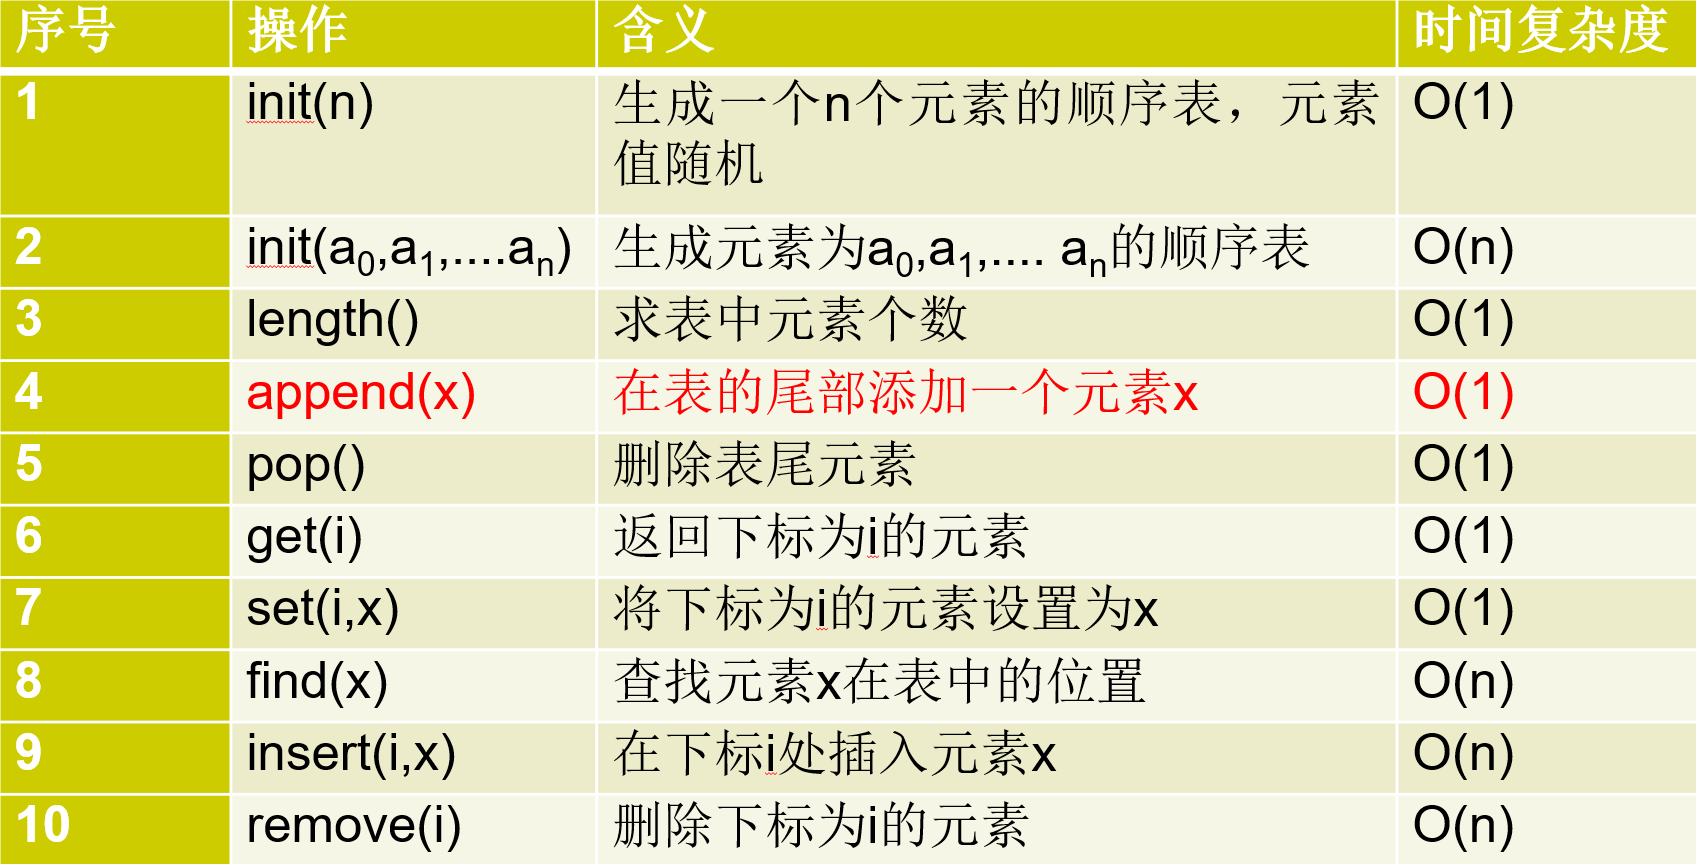
\includegraphics[width=\columnwidth]{images/顺序表支持的操作.png}

\subsubsection{顺序表的 {\ttfamily append} 的$O(1)$复杂度的实现}
总是分配多于实际元素个数的空间(容量大于元素个数)


元素个数小于容量时,\verb|append| 操作复杂度 $O(1)$


元素个数等于容量时,\verb|append| 导致重新分配空间,且要拷贝原有元素到新空间,复杂度 $O(n)$

重新分配空间时,新容量为旧容量的$k$倍($k>1$且固定),可确保 \verb|append| 操作的平均复杂度是$O(1)$。Python的 \verb|list| 取$k=1.2$左右。

\subsection{链表}
元素在内存中并非连续存放,元素之间通过指针链接起来

每个结点除了元素,还有 \verb|next| 指针,指向后继

不支持随机访问。访问第 \verb|i| 个元素,复杂度为$O(n)$

已经找到插入或删除位置的情况下,插入和删除元素的复杂度$O(1)$,且不需要复制或移动结点

有多种形式:单链表、循环单链表、双向链表、循环双向链表

\subsubsection{单链表}
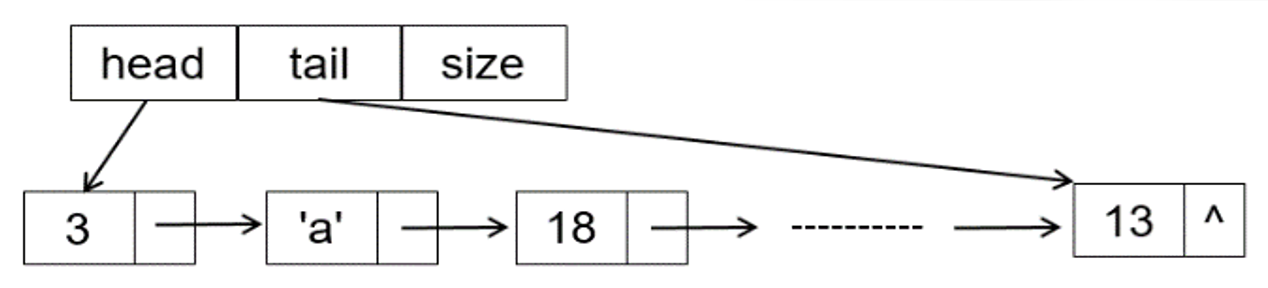
\includegraphics[width=\columnwidth]{images/单链表.png}
\begin{lstlisting}[style=python]
class LinkList:
	class Node: #表结点
		def __init__(self, data, next=None):
			self.data, self.next = data, next
	def __init__(self):
		self.head = self.tail = None
		self.size = 0

	def printList(self): #打印全部结点
		ptr = self.head
		while ptr is not None: 
			print(ptr.data, end=",")
			ptr = ptr.next

	def insert(self,p,data): #在结点p后面插入元素
		nd = LinkList.Node(data,None)
		if self.tail is p:  # 新增的结点是新表尾
			self.tail = nd
		nd.next = p.next
		p.next = nd
		self.size += 1
        
	def delete(self,p):  #删除p后面的结点
		if self.tail is p.next:
			self.tail = p
		p.next = p.next.next
		self.size -= 1

	#结点空间会被Python自动回收

\end{lstlisting}

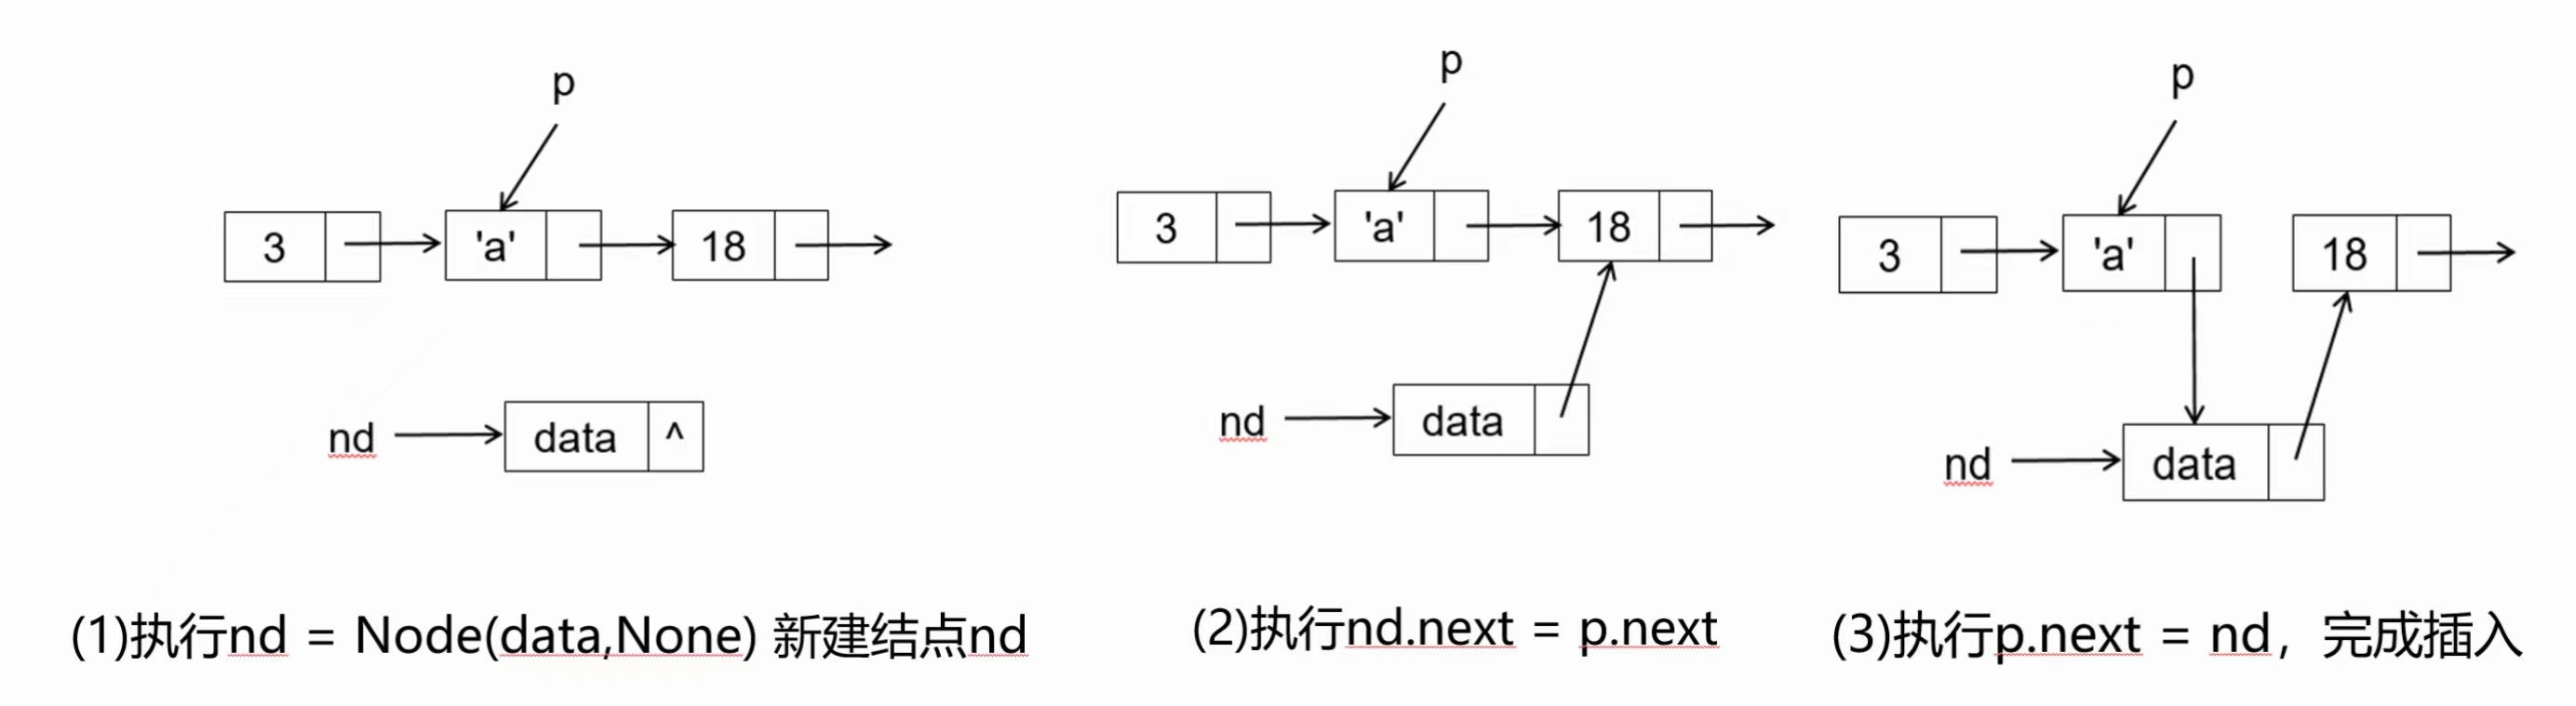
\includegraphics[width=\columnwidth]{images/单链表添加.jpg}

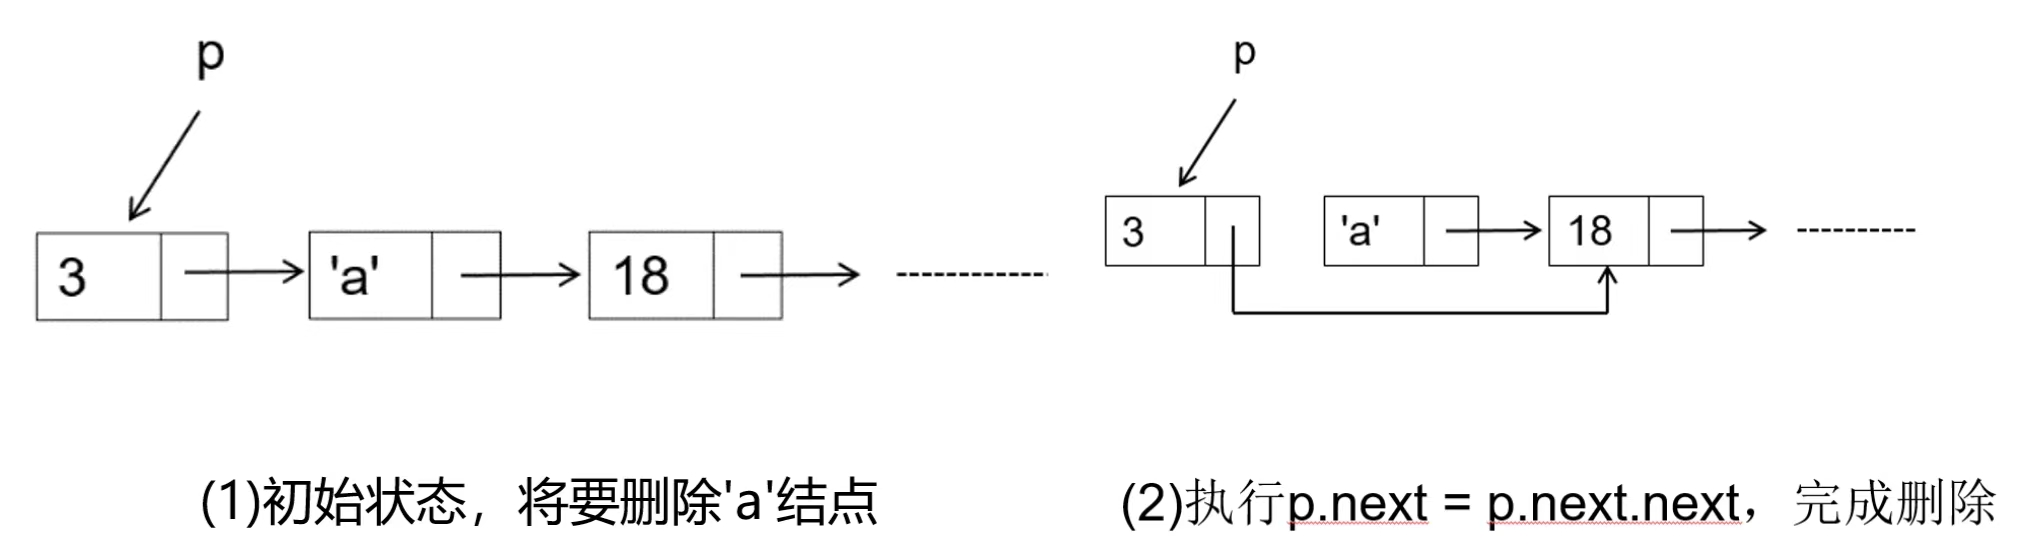
\includegraphics[width=\columnwidth]{images/单链表删除.jpg}

判断变量是否为 \verb|None|,应写 \verb|p is None, p is not None|
最好不要写 \verb|p == None, p != None|

\begin{lstlisting}[style=python]
	def popFront(self): #删除前端元素
		if self.head is None:
			raise \ 
		  Exception("Popping front for Empty link list.")
		else:
			self.head = self.head.next
			self.size -= 1
			if self.size == 0:
				self.head = self.tail = None
	def pushBack(self,data): #在尾部添加元素
		if self.size == 0:
			self.pushFront(data)
		else:
			self.insert(self.tail,data)

	def pushFront(self,data): #在链表前端插入一个元素data
		nd = LinkList.Node(data, self.head)
		self.head = nd
		self.size += 1
		if self.tail is None:
			self.tail = nd

	def clear(self):
		self.head = self.tail = None
		self.size = 0
	def __iter__(self):
		self.ptr = self.head
		return self
	def __next__(self):
		if self.ptr is None:
			raise StopIteration()  # 引发异常
		else:
			data = self.ptr.data
			self.ptr = self.ptr.next
			return data

\end{lstlisting}

\begin{lstlisting}[style=python]
linkLst = LinkList()
linkLst.pushFront(0)
linkLst.pushFront(1)
for i in range(2,5):
	linkLst.pushBack(i)
for x in linkLst:	#>>1,0,2,3,4,
	print(x,end=",")

\end{lstlisting}
上述实现方式没有实现“隐藏”,不是很好的实现方式

\subsubsection{带头结点的单链表}
为避免链表为空是做特殊处理,可以为链表增加一个空闲头结点

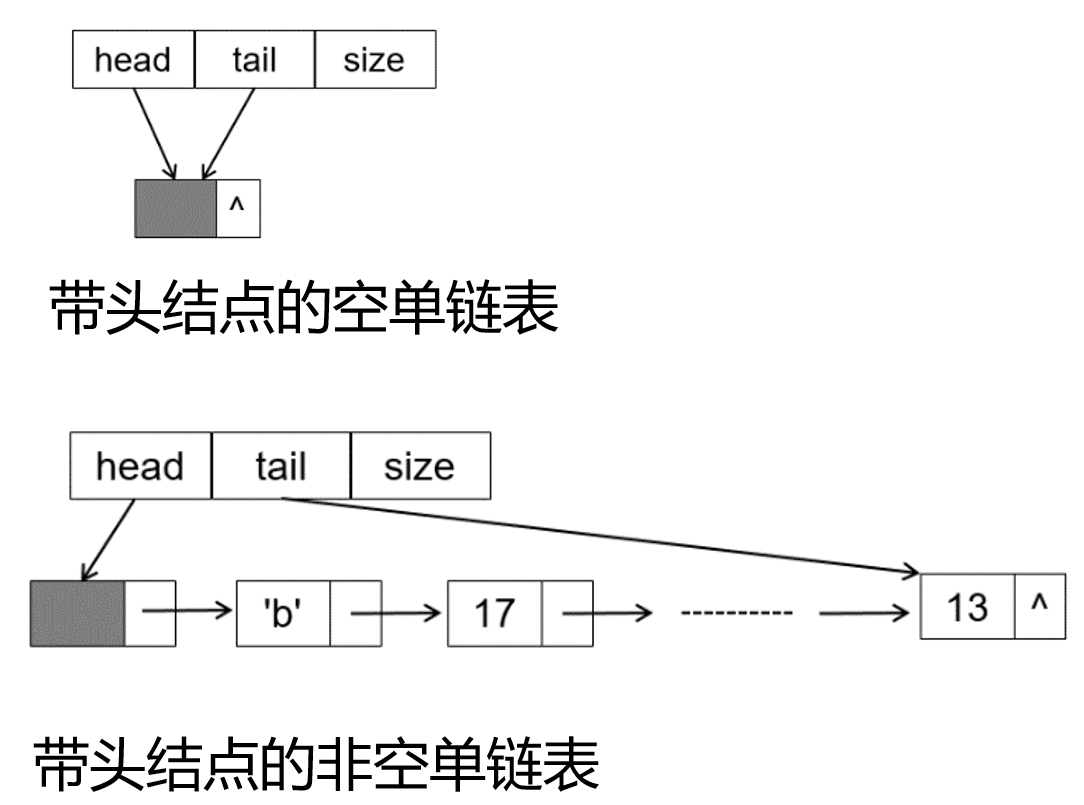
\includegraphics[width=.8\columnwidth]{images/头结点单链表.png}

\begin{lstlisting}[style=python]
class LinkList:
	def __init__(self):
		self.head = self.tail =  LinkList.Node(None,None)
		self.size = 0

\end{lstlisting}

\subsubsection{循环单链表}
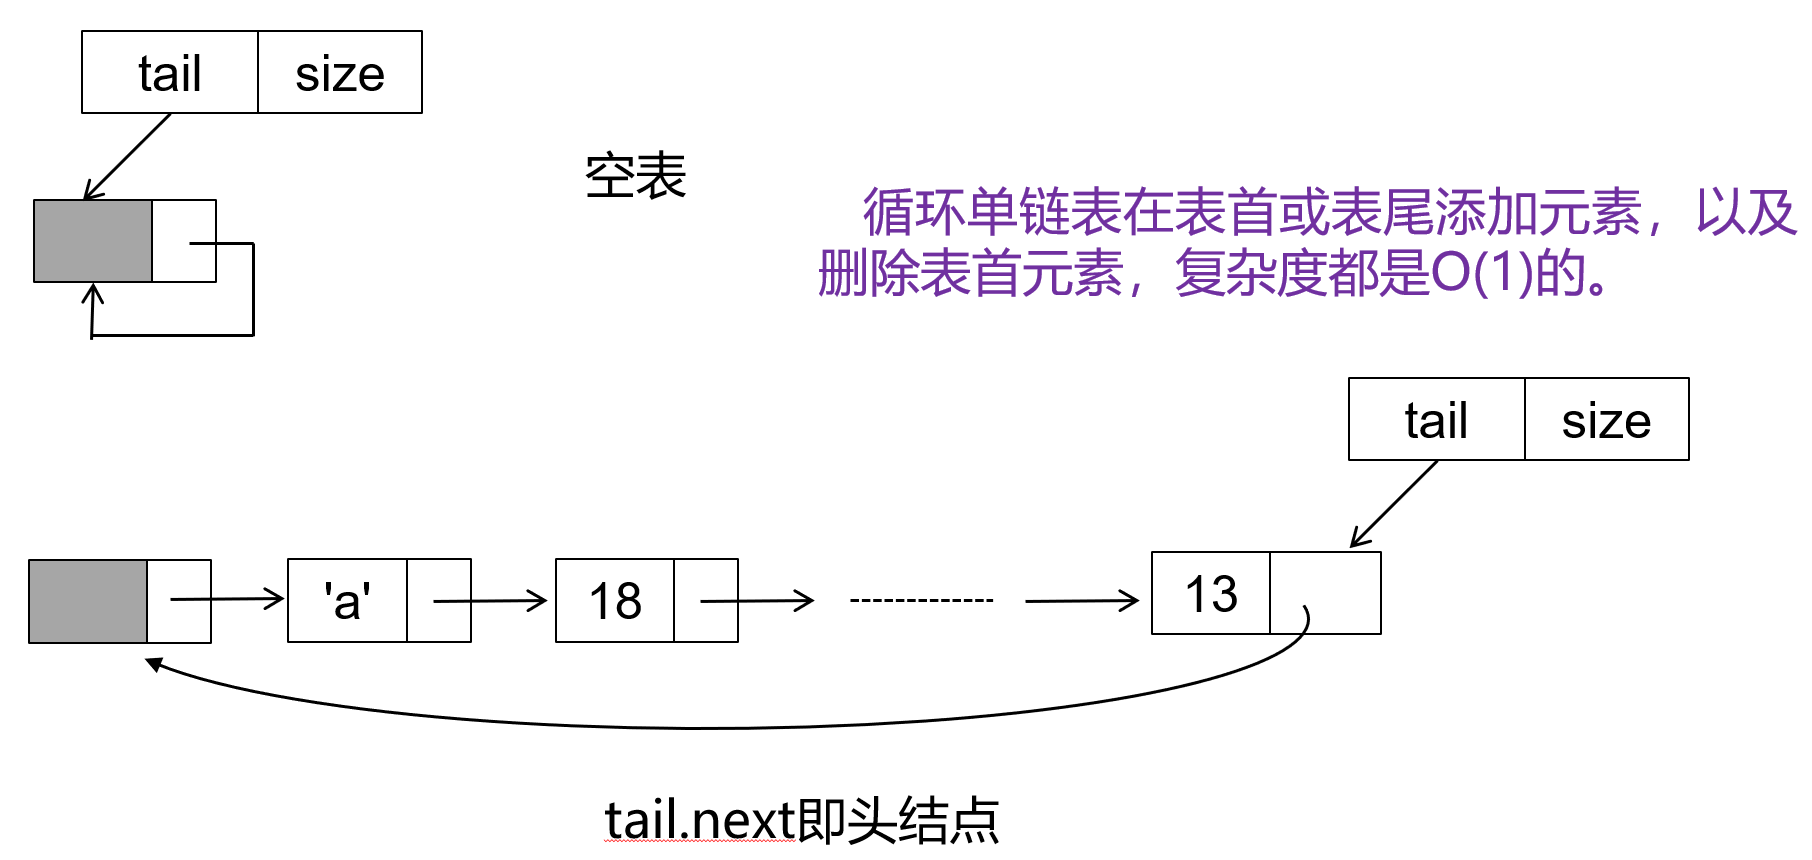
\includegraphics[width=\columnwidth]{images/循环单链表.png}

\subsubsection{双向链表}
每个结点有 \verb|text| 指针指向后继,有 \verb|prev| 指针指向前驱

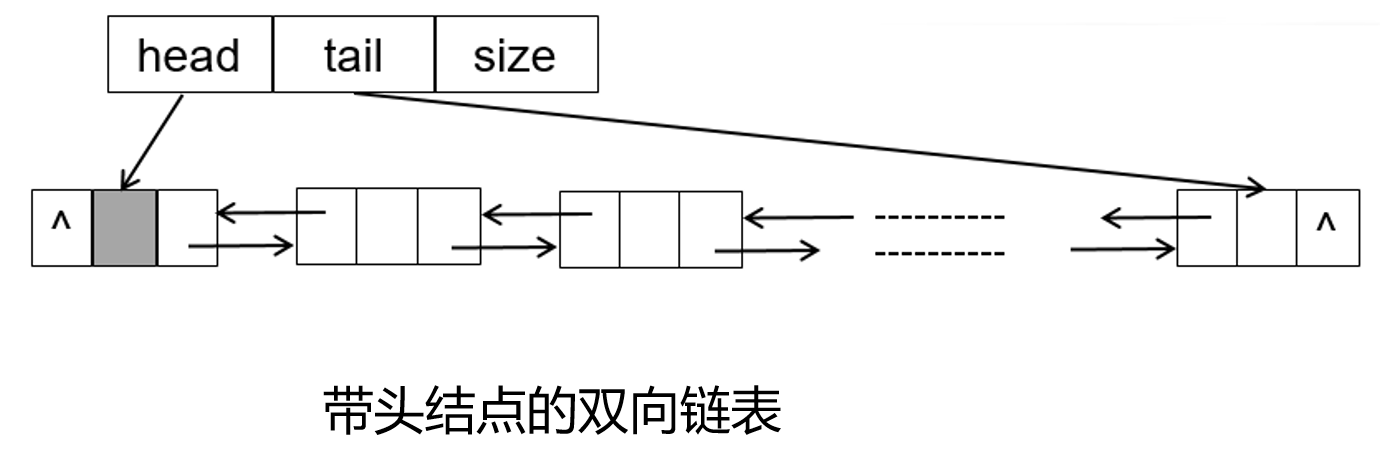
\includegraphics[width=\columnwidth]{images/带头结点的双向链表.png}

\begin{lstlisting}[style=python]
class DoubleLinkList:
	class _Node:
		def __init__(self, data, prev=None, next=None):
			self.data, self.prev, self.next = data, prev, next
\end{lstlisting}

在结点 \verb|p| 后面插入新结点 \verb|nd|

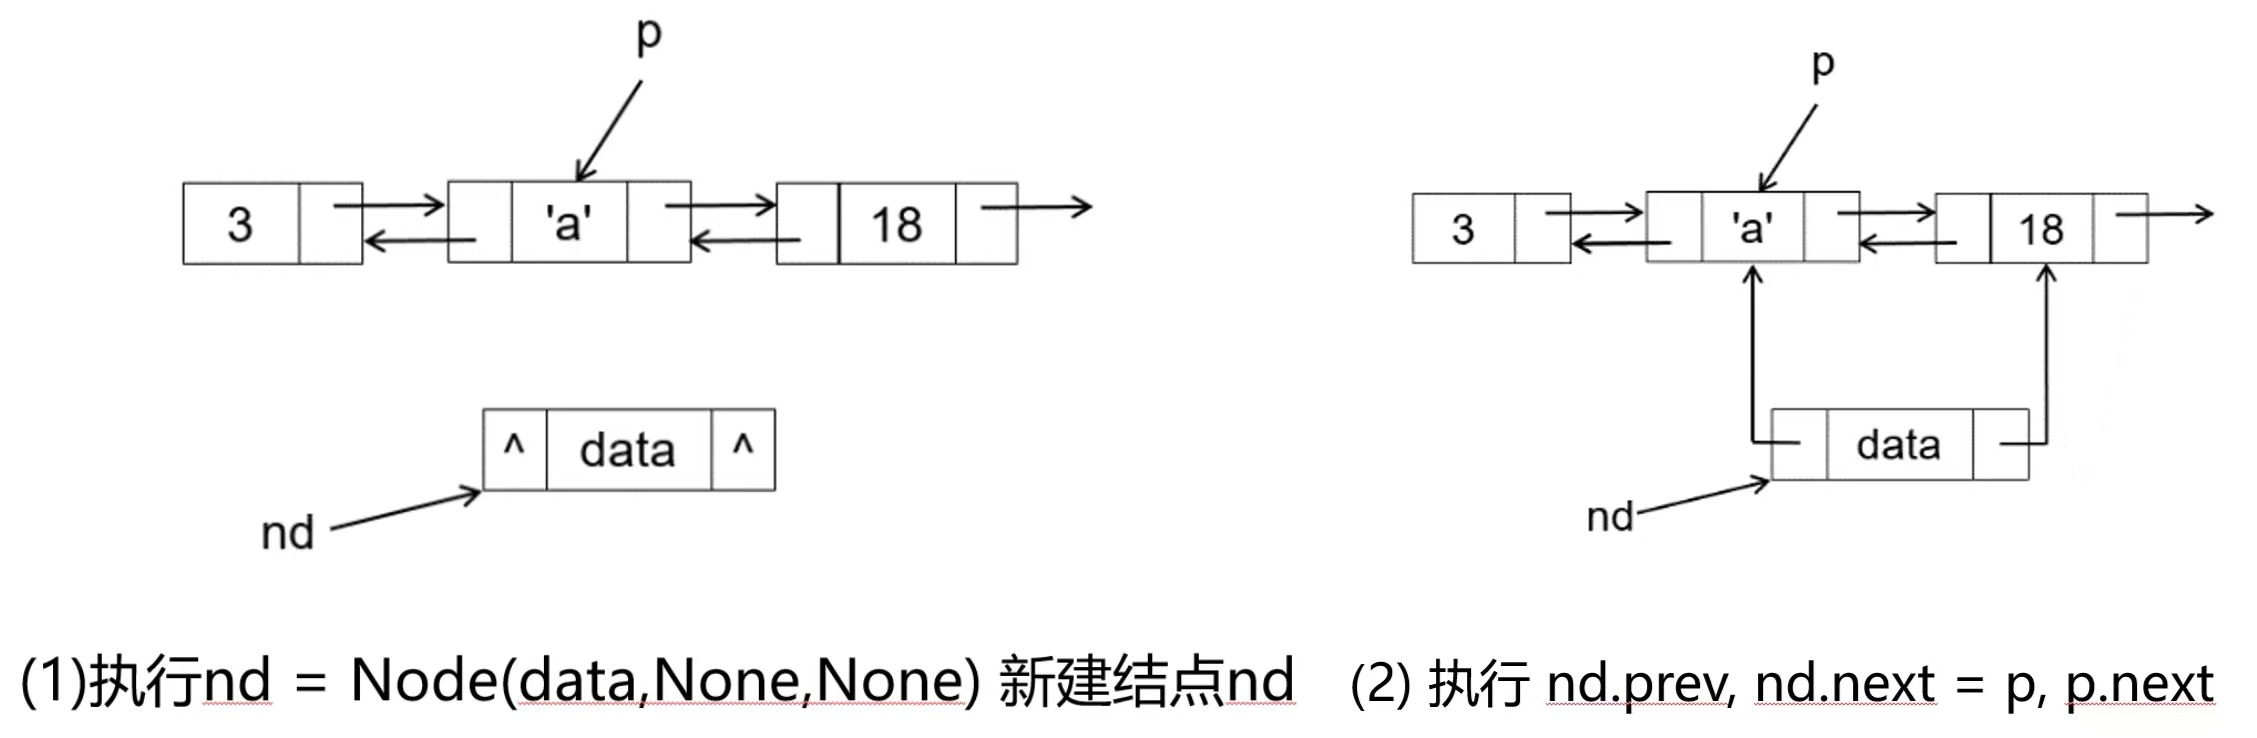
\includegraphics[width=\columnwidth]{images/双向链表插入1.jpg}
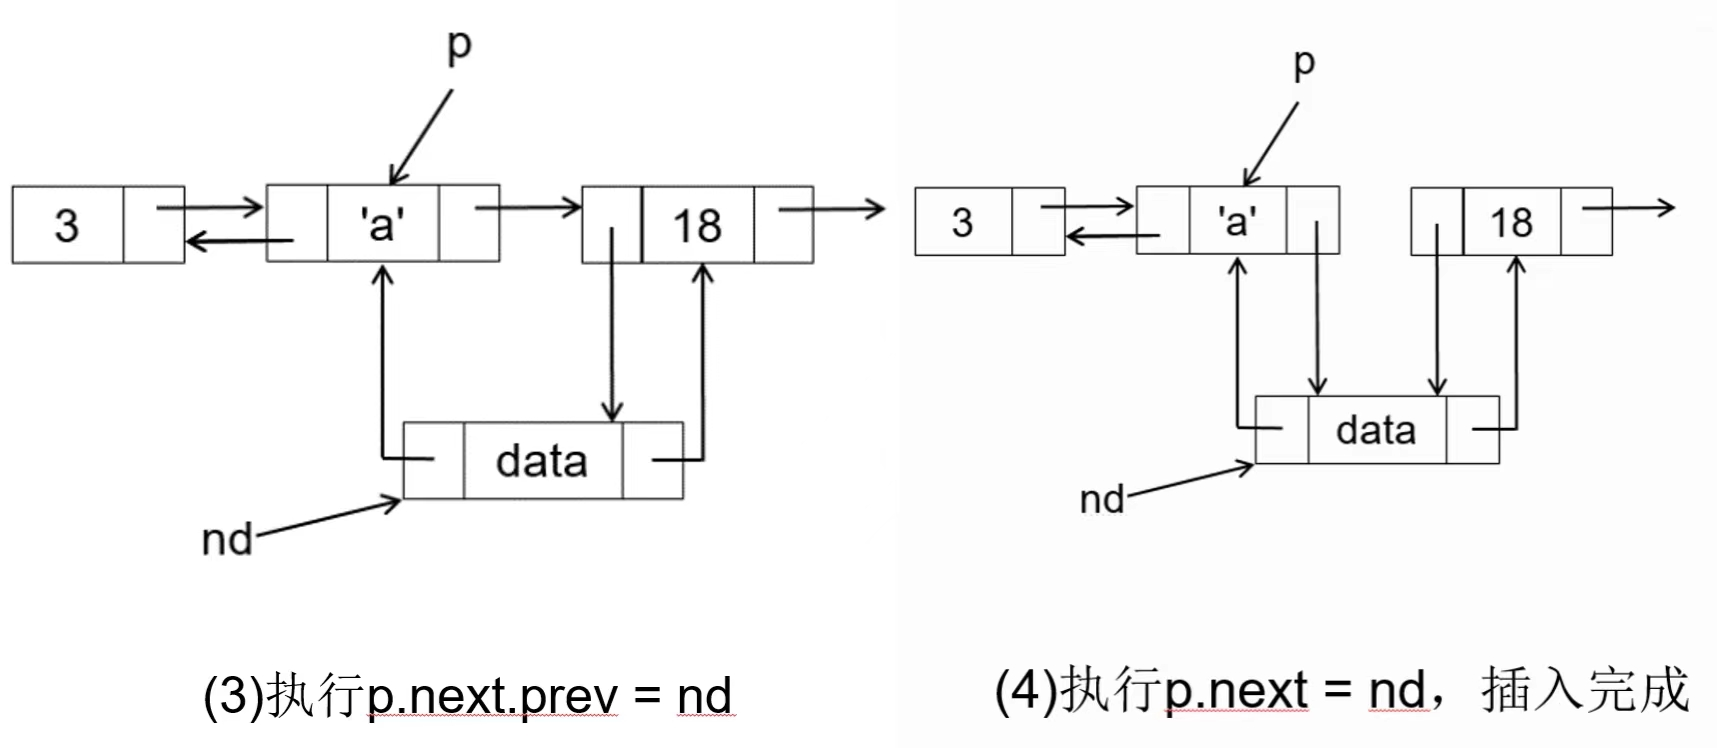
\includegraphics[width=\columnwidth]{images/双向链表插入2.jpg}

删除结点 \verb|p|

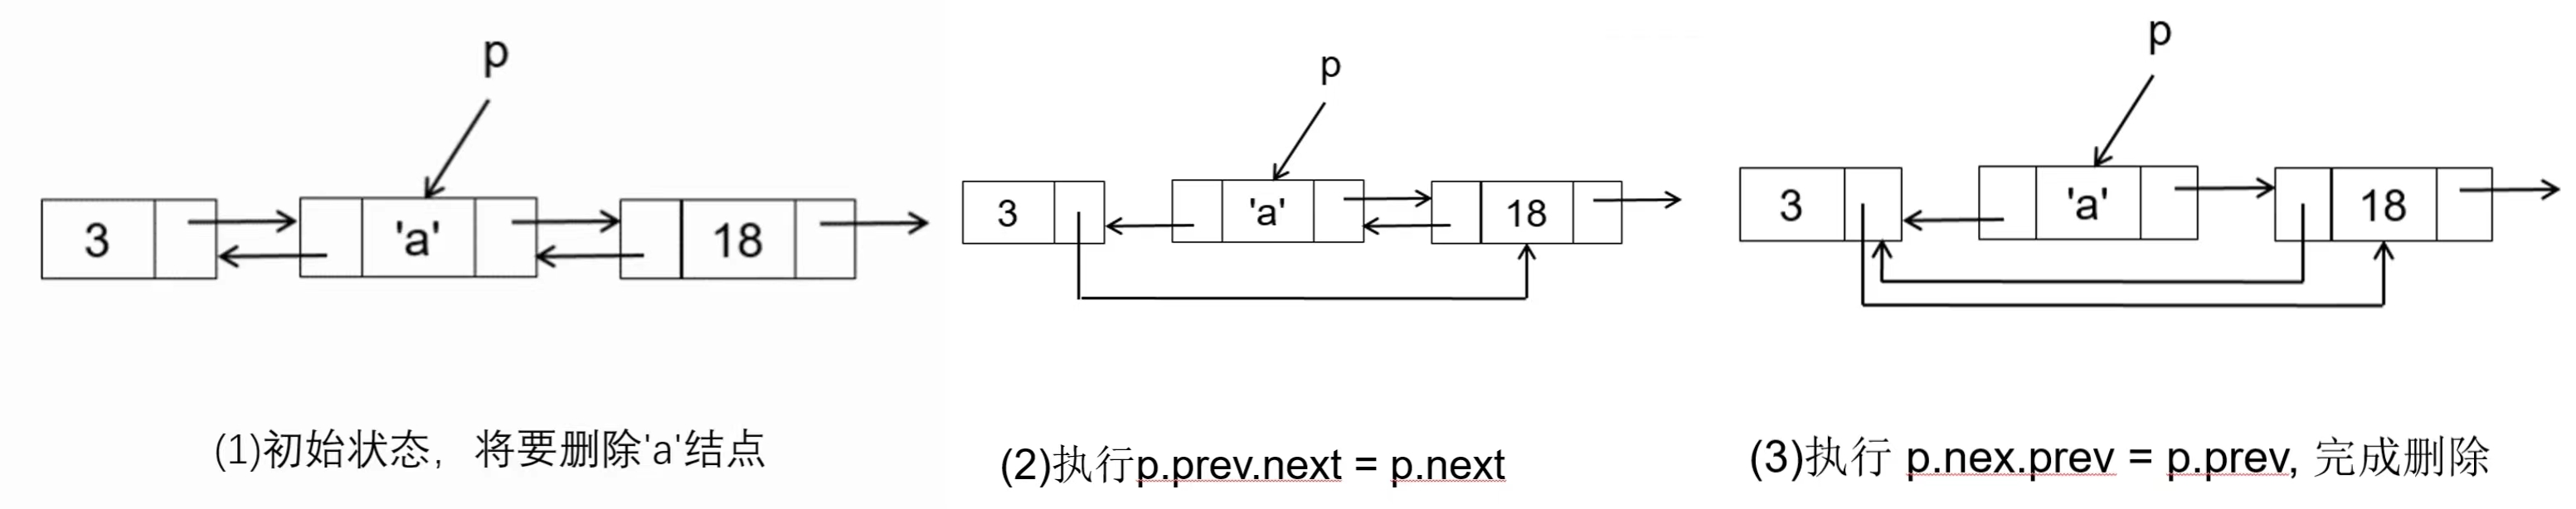
\includegraphics[width=\columnwidth]{images/双向链表删除.jpg}

双向链表实现
\begin{lstlisting}[style=python]
class DoubleLinkList:
	class _Node:
		def __init__(self, data, prev=None, next=None):
			self.data, self.prev, self.next = data, prev, next

	class _Iterator: 
		def __init__(self,p):
			self.ptr = p
		def getData(self):
			return self.ptr.data
		def setData(self,data):
			self.ptr.data = data
		def __next__(self):
			self.ptr = self.ptr.next
			if self.ptr is None:
				return None
			else:
				return DoubleLinkList._Iterator(self.ptr)
        def prev(self):
			self.ptr = self.ptr.prev
			return DoubleLinkList._Iterator(self.ptr)

	def __init__(self):
		self._head = self._tail = \
			DoubleLinkList._Node(None,None,None)
		self._size = 0

	def _insert(self,p,data):
		nd = DoubleLinkList._Node(data,p,p.next)
		if self._tail is p:  # 新增的结点是新表尾
			self._tail = nd
		if p.next:
			p.next.prev = nd
		p.next = nd
		self._size += 1

	def _delete(self,p):  #删除结点p
		if self._size == 0 or p is self._head:
			raise Exception("Illegal deleting.")
		else:
			p.prev.next = p.next
			if p.next: #如果p有后继
				p.next.prev = p.prev
			if self._tail is p:
				self._tail = p.prev
			self._size -= 1

	def clear(self):
		self._tail = self._head
		self._head.next = self._head.prev = None
		self.size = 0

	def begin(self):
		return DoubleLinkList._Iterator(self._head.next)

	def end(self):
		return None

	def insert(self,i,data): #在迭代器i指向的结点后面插入元素
		self._insert(i.ptr,data)

	def delete(self, i):  # 删除迭代器i指向的结点
		self._delete(i.ptr)

	def pushFront(self,data): #在链表前端插入一个元素
		self._insert(self._head,data)

	def popFront(self):
		self._delete(self._head.next)

	def pushBack(self,data):
		self._insert(self._tail,data)

	def popBack(self):
		self._delete(self._tail)

	def __iter__(self):
		self.ptr = self._head.next
		return self

	def __next__(self):
		if self.ptr is None:
			raise StopIteration()  # 引发异常
		else:
			data = self.ptr.data
			self.ptr = self.ptr.next
			return data

	def find(self,val): #查找元素val,找到返回迭代器,找不到返回None
		ptr = self._head.next
		while ptr is not None:
			if ptr.data == val:
				return DoubleLinkList._Iterator(ptr)
			ptr = ptr.next
		return self.end()

	def printList(self):
		ptr = self._head.next
		while ptr is not None:
			print(ptr.data,end=",")
			ptr = ptr.next

linkLst = DoubleLinkList()
for i in range(5):
	linkLst.pushBack(i)
i = linkLst.begin()
while i != linkLst.end(): #>>0,1,2,3,4,
	print(i.getData(),end = ",")
	i = next(i)
print()
i = linkLst.find(3)
i.setData(300)
linkLst.printList()  #>>0,1,2,300,4,
print()
linkLst.insert(i,6000) #在i后面插入6000
linkLst.printList() #>>0,1,2,300,6000,4,
print()
linkLst.delete(i)
linkLst.printList() #>>0,1,2,6000,4,


\end{lstlisting}

\subsection{链表和顺序表的选择}
\subsubsection{顺序表}
中间插入太慢

\subsubsection{链表}
访问第 \verb|i| 个元素太慢

顺序访问也慢(现代计算机有cache,访问连续内存域比跳着访问内存区域快很多)

还多费空间

\subsubsection{结论}
尽量选用顺序表。比如栈和队列,都没必要用链表实现

基本只有在找到一个位置后反复要在该位置周围进行增删,才适合用链表

实际工作中几乎用不到链表


\section{枚举与二分法}
\subsection{二分法寻找答案的核心思想}
如果一个假设的答案成立,那就跳着试一个更优的假设答案看行不行;

如果一个假设的答案不成立,那就跳着试一个更差的假设答案看行不行。

必须每次验证假设答案,都可以把假设答案所在的区间缩小为上次的一半。


前提:单调性。一个假设答案不成立,则比它更优的假设答案肯定都不成立。

\subsection{二分查找函数}
写一个函数 \verb|BinarySeach|,在从小到大排序的列表 \verb|a| 里查找元素 \verb|p|,如果找到,则返回元素下标,如果找不到,则返回 \verb|None|。要求复杂度$O(\log(n))$

\begin{lstlisting}[style=python]
def binarySearch(a,p,key = lambda x : x): 
    L, R = 0,len(a)-1  #查找区间的左右端点,区间含右端点 
    while L <= R: #如果查找区间不为空就继续查找 
        mid = L+(R-L)//2 #取查找区间正中元素的下标 
        if key(p) < key(a[mid]): 
            R = mid - 1  #设置新的查找区间的右端点 
        elif key(a[mid]) < key(p): 
            L = mid + 1  # 设置新的查找区间的左端点 
        else:
            return mid 
    return None
\end{lstlisting}

\section{递归和分治}
\subsection{递归}
\subsubsection{递归的作用}
1) 替代多重循环进行枚举

2) 解决本来就是用递归形式定义的问题

3) 将问题分解为规模更小的子问题进行求解

……

\section{栈和队列}
\subsection{栈}
类似于子弹匣,后压进去的子弹,先射出去

支持四种操作:

	\begin{tabular}{ll}
        \verb|top()|		&返回栈顶元素\\
        \verb|push(x)|		&将 \verb|x| 压入栈中\\
        \verb|pop()|		&弹出并返回栈顶元素\\
        \verb|isEmpty()|	&看栈是否为空
    \end{tabular}

要求上面操作复杂度都是$O(1)$

用列表可以实现栈

四种操作的实现(\verb|stack| 为一个列表):

	\begin{tabular}{ll}
        \verb|top()|		&\verb|stack[-1]|\\
        \verb|push(x)|		&\verb|stack.append(x)|\\
        \verb|pop()|		&\verb|stack.pop()|\\
        \verb|isEmpty()|	&\verb|len(stack) == 0|\\
    \end{tabular}

\subsection{队列}
即排队的队列。只能一头进(\verb|push|),另一头出(\verb|pop|)。先进先出

要求进出的复杂度都是$O(1)$

如果用列表的 \verb|append| 进,\verb|pop(0)| 出,则出的复杂度为$O(n)$

\subsubsection{队列的实现方法一}
用足够大的列表实现,维护一个队头指针和队尾指针,初始:\verb|head=tail = 0|

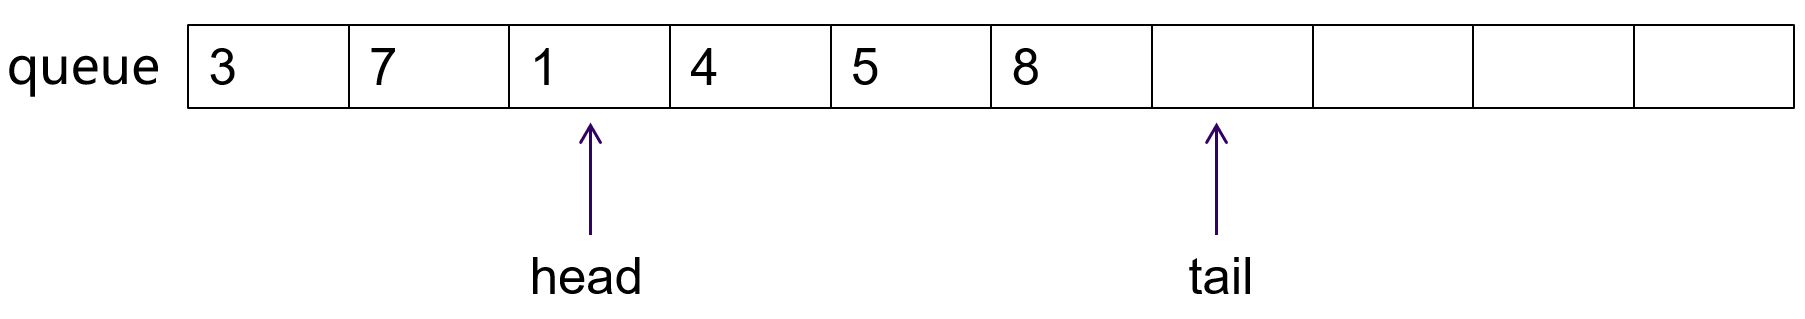
\includegraphics[width=\columnwidth]{images/队列1.png}

\verb|head| 指向队头元素,\verb|tail| 指向队尾元素的后面

\verb|push(x)| 的实现:

\verb|queue[tail] = x| 	

\verb|tail+=1|

\verb|pop()| 的实现:\verb|head += 1|

判断队列是否为空:\verb|head == tail|

\subsubsection{队列的实现方法二}
如果不想浪费空间开足够大的列表,而是想根据实际情况分配空间,则可以用列表+头尾循环法实现队列

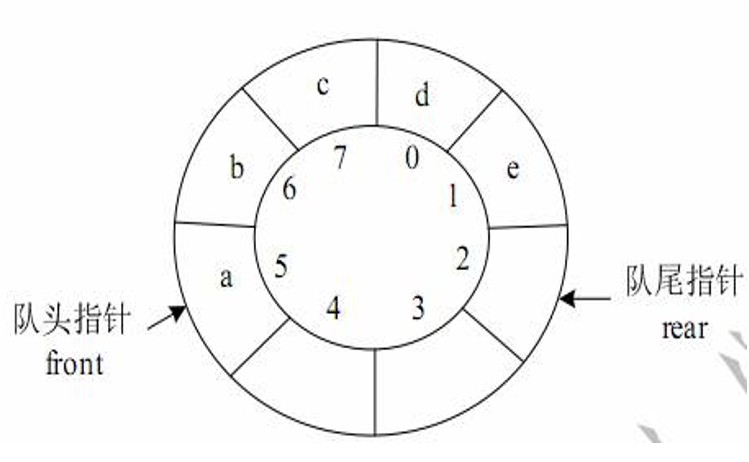
\includegraphics[width=\columnwidth]{images/队列2.png}

1) 预先开设一个 \verb|capacity| 个空元素的列表 \verb|queue|,\verb|head = tail = 0|

2) 列表没有装满的情况下:

\verb|push(x)| 的实现:

	\verb|queue[tail] = x|

	\verb|tail = (tail+1) % capacity|

\verb|pop()| 的实现:

	\verb|head =  (head+1) % capacity|

\verb|capacity| 可以是4,8,16.....

3) 如何判断队列是否为空:

    方法1:维护一个元素总数 \verb|size, size == 0| 即为空

    方法2:不维护 \verb|size|,浪费 \verb|queue| 中一个单元的存储空间

                 \verb|head == tail| 即为空

4) 如何判断队列是否为满:

    方法1:维护一个元素总数 \verb|size, size == capacity| 即为满

    方法2:不维护 \verb|size|, 浪费 \verb|queue| 中一个单元的存储空间,

	    \verb|(tail + 1) % capacity == head| 即为满

                 如果不浪费,就无法区分 \verb|head == tail| 是队列空导致,还是队列满导致


5) 若一个push操作后导致列表满:

i. 建一个大小是原列表$k$倍大的新列表($k>1$,可以取1.5,2.....)

ii. 将原列表内容全部拷贝到新列表,作为新队列

iii. 重新设置新列表的 \verb|head| 和 \verb|tail|   

iv. 原列表空间自动被Python解释器回收

导致队列满的 \verb|push| 的时间复杂度是$O(n)$。平均 \verb|push| 操作是 $O(1)$

Python列表 \verb|append| 做到$O(1)$的实现也是这种原理,且$k$取1.125,空间换时间

若每次增加空间只增加固定数量,比如20个单元,则 \verb|push| 平均复杂度还是$O(n)$

\begin{lstlisting}[style=python]
class Queue:
	_initC = 8		#存放队列的列表的初始容量
	_expandFactor = 1.5  #扩充容量时容量增加的倍数
	def __init__(self):
		self._q = [None for i in range(Queue._initC)]
		self._size = 0				    #队列元素个数
		self._capacity = Queue._initC #队列最大容量
		self._head = self._rear = 0
	def isEmpty(self):
		return self._size == 0
	def front(self):  #看队头元素。空队列导致re
		if self._size == 0:
			raise Exception("Queue is empty")
		return self._q[self._head]
	def back(self):   #看队尾元素,空队列导致re
		if self._size == 0:
			raise Exception("Queue is empty")
		if self._rear > 0:
			return self._q[self._rear - 1]
		else:
			return self._q[-1]
	def push(self,x):
		if self._size == self._capacity:
			tmp = [None for i in range(
					int(self._capacity*Queue._expandFactor))]
			k = 0
			while k < self._size:
				tmp[k] = self._q[self._head]
				self._head = (self._head + 1) % self._capacity
				k += 1
			self._q = tmp  #原来self._q的空间会被Python自动释放
			self._q[k] = x
			self._head,self._rear = 0,k+1
			self._capacity = int(
					self._capacity*Queue._expandFactor)
		else:
			self._q[self._rear] = x
			self._rear = (self._rear + 1) % self._capacity
		self._size += 1
	def pop(self):
		if self._size == 0:
			raise Exception("Queue is empty")
		self._size -= 1
		self._head = (self._head + 1) % len(self._q)

q = Queue()
for i in range(1,314):
	q.push(i)
	print(q.back(),end=",")
print()
while not q.isEmpty():
	print(q.front(),end=",")
	q.pop()


\end{lstlisting}


\subsubsection{用两个栈实现一个队列}


执行 \verb|push(x)| 操作时,将 \verb|x| 压入栈 \verb|inStack|,执行 \verb|pop()| 或 \verb|front()| 操作时,看另一个栈 \verb|outStack| 是否为空,若不为空,弹出栈顶元素或访问栈顶元素即可;若为空,则先将 \verb|inStack| 中的全部元素弹出并依次压入 \verb|outStack|,然后再弹出或访问 \verb|outStack| 的栈顶元素。



由于每个元素最多出入 \verb|inStack| 各一次,出入 \verb|outStack| 各一次,所以 \verb|pop| 和 \verb|front| 操作的平均复杂度是 $O(1)$的。


\subsubsection{Python中的队列}
\verb|collections| 库中的 \verb|deque| 是双向队列,可以像普通列表一样访问,且在两端进出,复杂度都是 $O(1)$。

\begin{lstlisting}[style=python]
import collections
dq = collections.deque()
dq.append('a') #右边入队
dq.appendleft(2) #左边入队
dq.extend([100,200]) #右边加入100,200
dq.extendleft(['c','d']) #左边依次加入 'c','d'
print(dq.pop()) #>>200 右边出队
print(dq.popleft()) #>>d 左边出队
print(dq.count('a')) #>>1
dq.remove('c') 
print(dq)	#>>deque([2, 'a', 100])
dq.reverse() 
print(dq)	#>>deque([100, 'a', 2])
print(dq[0],dq[-1],dq[1]) #>>100 2 a
print(len(dq)) #>>3
dq.clear()				#清空队列
print(len(dq),dq)		#>0 deque([])

\end{lstlisting}

\section{二叉树}
\subsection{二叉树的概念及性质}
\subsubsection{二叉树的定义}
1) 二叉树是有限个元素的集合。

2) 空集合是一个二叉树,称为空二叉树。

3) 一个元素(称其为“根”或“根结点”),加上一个被称为“左子树”的二叉树,和一个被称为“右子树”的二叉树,就能形成一个新的二叉树。要求根、左子树和右子树三者没有公共元素。

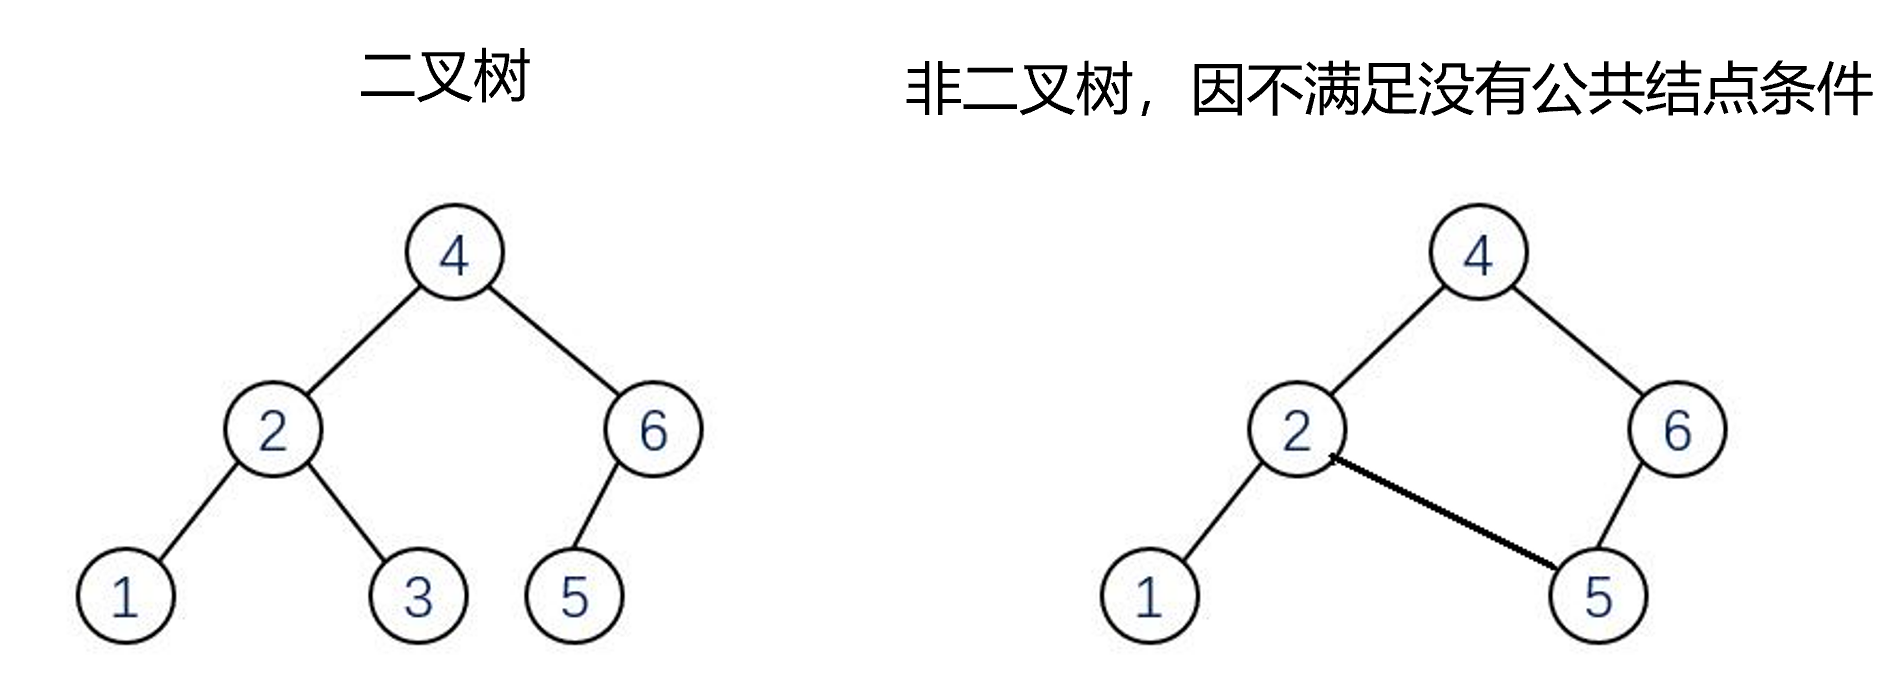
\includegraphics[width=\columnwidth]{images/二叉树定义.png}

\subsubsection{二叉树的左右子树是有区别的}

以下是两棵不同的二叉树:

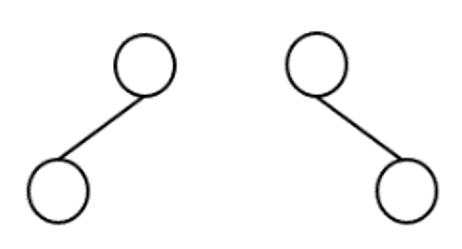
\includegraphics[width=.5\columnwidth]{images/两个不同二叉树.png}

以下是三棵不同的二叉树:

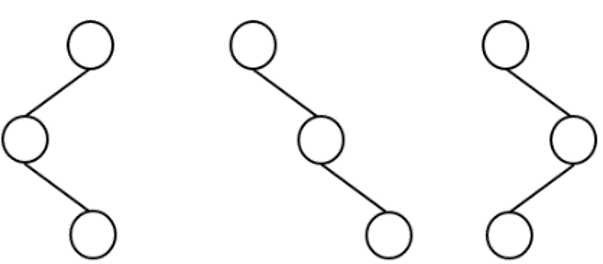
\includegraphics[width=.5\columnwidth]{images/三颗不同二叉树.png}

\subsubsection{二叉树的相关概念}
二叉树的的元素称为“结点”。结点由三部分组成:数据、左子结点指针、右子结点指针。

结点的度(degree):结点的非空子树数目。也可以说是结点的子结点数目。

叶结点(leaf node):度为 \verb|0| 的结点。

分支结点:度不为 \verb|0| 的结点。即除叶子以外的其他结点。也叫内部结点。

兄弟结点(sibling):父结点相同的两个结点,互为兄弟结点。

结点的层次(level):树根是第 \verb|0| 层的。如果一个结点是第 \verb|n| 层的,则其子结点就是第 \verb|n+1| 层的。

结点的深度(depth):即结点的层次。

祖先(ancestor):

	1)	父结点是子结点的祖先

	2)	若 \verb|a| 是 \verb|b| 的祖先,\verb|b| 是 \verb|c| 的祖先,则 \verb|a| 是 \verb|c| 的祖先。

子孙(descendant):也叫后代。若结点 \verb|a| 是结点 \verb|b| 的祖先,则结点 \verb|b| 就是结点 \verb|a| 的后代。

边:若 \verb|a| 是 \verb|b| 的父结点,则对子 \verb|<a,b>| 就是a到b的边。在图上表现为连接父结点和子结点之间的线段。

二叉树的高度(height):二叉树的高度就是结点的最大层次数。只有一个结点的二叉树,高度是0。结点一共有n层,高度就是n-1。

完美二叉树(perfect binary tree):每一层结点数目都达到最大。即第 \verb|i| 层有$2^i$个结点。高为$h$的完美二叉树,有$2^{h+1} -1$个结点

满二叉树(full binary tree):没有1度结点的二叉树

完全二叉树(complete binary tree):除最后一层外,其余层的结点数目均达到最大。而且,最后一层结点若不满,则缺的结点定是在最右边的连续若干个。

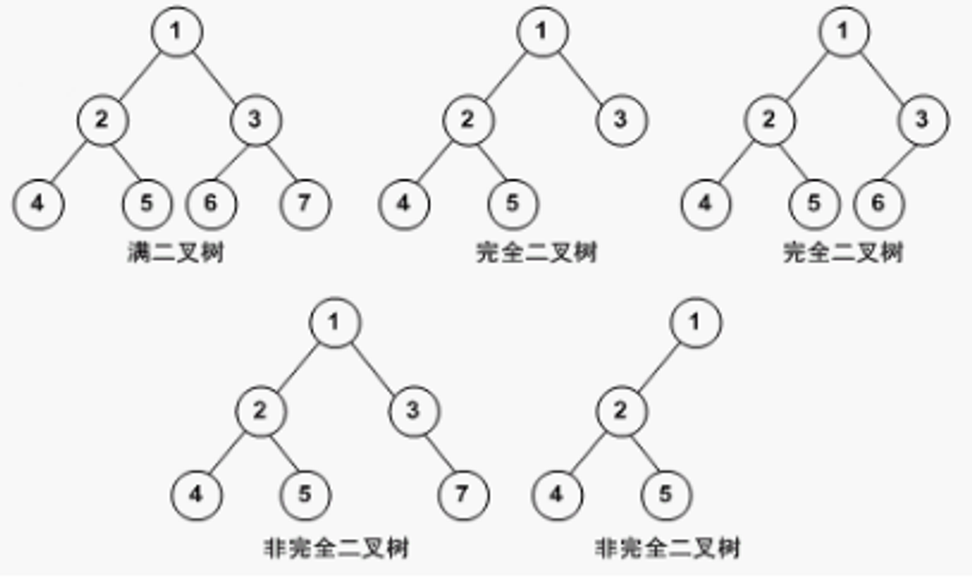
\includegraphics[width=.8\columnwidth]{images/完全二叉树.png}

\subsubsection{二叉树的性质}
1) 第 $i$层最个多$2^i$个结点

2) 高为$h$的二叉树结点总数最多$2^{h+1}-1$

3) 结点数为$n$的树,边的数目为$n-1$

4) $n$个结点的非空二叉树至少有$\log_2(n+1)$层结点,即高度至少为$\log_2(n+1)- 1$

5) 在任意一棵二叉树中,若叶子结点的个数为$n_0$,度为2的结点个数为$n_2$,则$n_0=n_2+1$。

6) 非空满二叉树叶结点数目等于分支结点数目加1。

7) 非空二叉树中的空子树数目等于其结点数目加1。

\subsubsection{完全二叉树的性质}
1) 完全二叉树中的1度结点数目为0个或1个

2) 有$n$个结点的完全二叉树有$(n+1)/2$个叶结点。

3) 有$n$个叶结点的完全二叉树有$2n$或$2n-1$个结点(两种都可以构建)

4) 有$n$个结点的非空完全二叉树的高度为$\log_2(n+1)-1$。即:有$n$个结点的非空完全二叉树共有$\log_2(n+1)$层结点。

5) 可以用列表存放完全二叉树的结点,不需要左右子结点指针。下标为i的结点的左子结点下标是 \verb|2*i+1|, 右子结点是 \verb|2*i+2| (根下标为0)。下标为 \verb|i| 的元素,其父结点的下标就是 \verb|(i-1)//2| 

\subsection{二叉树的实现}

\begin{lstlisting}[style=python]
class BinaryTree:
	def __init__(self,data,left = None,right = None):
		self.data,self.left,self.right = data,left,right
	def addLeft(self,tree): #tree是一个二叉树
		self.left = tree
	def addRight(self,tree): #tree是一个二叉树
		self.right = tree

\end{lstlisting}

\subsubsection{二叉树的列表实现方法}
二叉树是一个三个元素的列表 \verb|X|

\verb|X[0]| 是根结点的数据,\verb|X[1]|,\verb|X[2]| 是右子树。如果没有左子树,\verb|X[1]| 就是空表 \verb|[]|,如果没有右子树,\verb|X[2]| 就是空表。

叶子结点为:\verb|[data,[],[]]|

\begin{lstlisting}[style=python]
[0,
    [1,
	[3,[],[]],
	[4,[],[]] ],
    [2,
	[5,[],[]],
	[6,[],[]] ]
]
即:[0, [1, [3, [], []], [4, [], []]], [2, [5, [], []], [6, [], []]]]


\end{lstlisting}

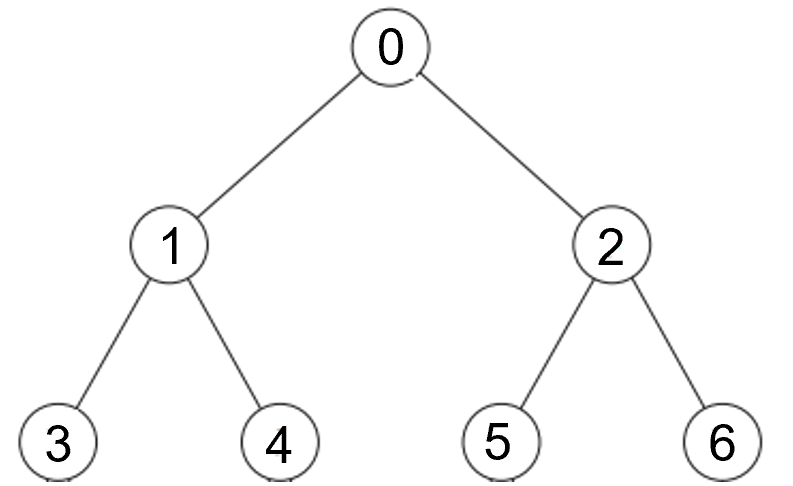
\includegraphics[width=.5\columnwidth]{images/二叉树列表实现.png}

\begin{lstlisting}[style=python]
class BinaryTree:
	def __init__(self,data,left = [],right = []):
		self.treeList = [data,left,right]
	def addLeft(self,tree):
		self.treeList[1] = tree.treeList
	def addRight(self,tree):
		self.treeList[2] = tree.treeList

\end{lstlisting}

\subsubsection{二叉树的遍历}
广度优先遍历:使用队列,按层遍历

深度优先遍历:编写递归函数

前序遍历过程:1)访问根结点 2)前序遍历左子树 3)前序遍历右子树。

中序遍历过程:1)中序遍历左子树 2)访问根结点 3)中序遍历右子树。

后序遍历过程:1)后序遍历左子树 2)后序遍历右子树 3)访问根结点。 

“访问”指的是对结点进行某种具体操作,比如输出其值、修改其值等。

遍历只需要访问每个结点一次,因此复杂度$O(n)$。$n$是总结点数目。

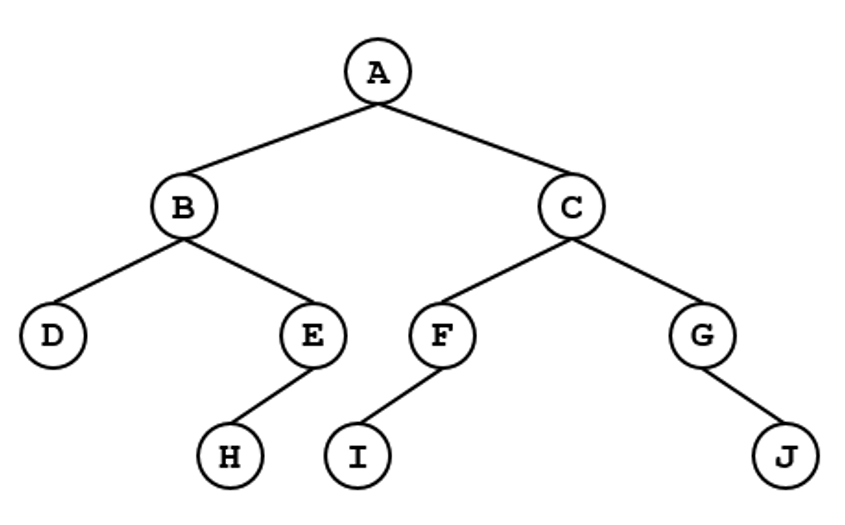
\includegraphics[width=.5\columnwidth]{images/二叉树的遍历.png}

前序遍历访问序列:ABDEHCFIGJ

中序遍历访问序列:DBHEAIFCGJ

后续遍历访问序列:DHEBIFJGCA

按层遍历访问序列:ABCDEFGHIJ

\begin{lstlisting}[style=python]
class BinaryTree:
	def __init__(self,data,left = None,right = None):
		self.data,self.left,self.right = data,left,right
	def addLeft(self,tree): #tree是一个二叉树
		self.left = tree
	def addRight(self,tree): #tree是一个二叉树
		self.right = tree
	def preorderTraversal(self, op): #前序遍历,op是函数,表示操作
		op(self)	#访问根结点
		if self.left:	#左子树不为空
			self.left.preorderTraversal(op) #遍历左子树
		if self.right:
			self.right.preorderTraversal(op) #遍历右子树
	def inorderTraversal(self, op): #中序遍历
		if self.left:
			self.left.inorderTraversal( op)
		op(self)
		if self.right:
			self.right.inorderTraversal(op)
	def postorderTraversal(self, op): #后序遍历
		if self.left:
			self.left.postorderTraversal(op)
		if self.right:
			self.right.postorderTraversal(op)
		op(self)
	def bfsTraversal(self,op): #按层次遍历
		import collections
		dq = collections.deque()
		dq.append(self)
		while len(dq) > 0:
			nd = dq.popleft()
			op(nd)
			if nd.left:
				dq.append(nd.left)
			if nd.right:
				dq.append(nd.right)

\end{lstlisting}

用法:

\begin{lstlisting}[style=python]
tree.preorderTraversal(lambda x: print(x.data,end="")
tree.preorderTraversal(lambda x: x.data+=100)

\end{lstlisting}

\subsubsection{遍历序列和二叉树}
1) 仅凭一种遍历序列(前序、后序、中序),不能确定二叉树的样子

2) 给出一棵二叉树的前序遍历序列,和后序遍历序列,依然不能确定这棵树的样子

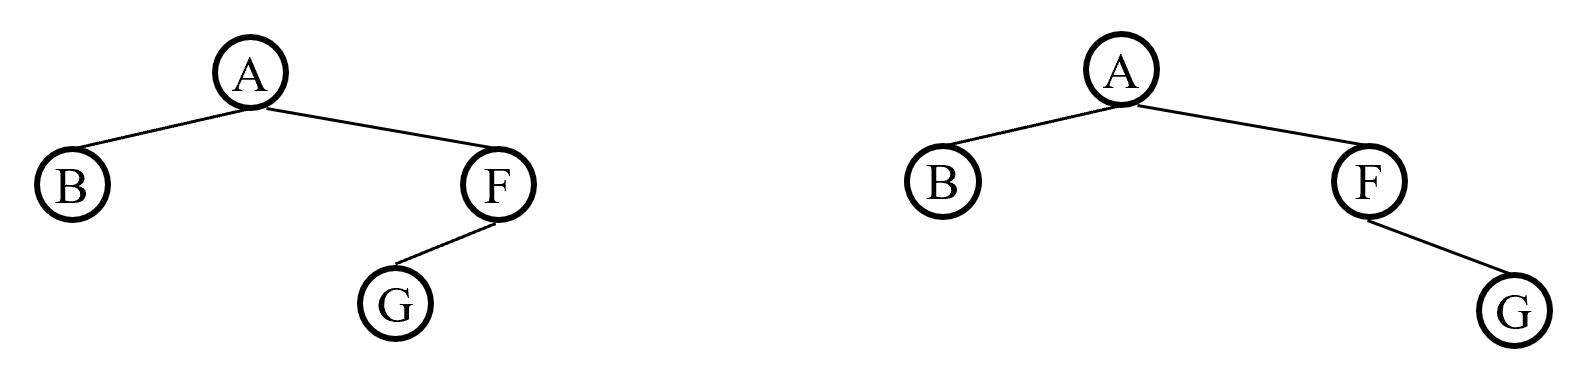
\includegraphics[width=.5\columnwidth]{images/遍历结果相同的不同二叉树.png}

上面两棵二叉树有相同前序序列和中序序列

给出一棵二叉树的中序遍历序列,再加上前序序列,或后序序列,就可以确定树的样子

\subsection{哈夫曼树(最优二叉树)}
给定$n$个结点,结点$i$有权值$W_i$。要求构造一棵二叉树,叶子结点为给定的结点,且
\begin{equation*}
	\text{WPL}=\sum_{i=1}^{n}W_i L_i
\end{equation*}
最小。$L_i$ 是结点$i$到树根的路径的长度。WPL: Weighted Path Length of Tree


最优二叉树也叫哈夫曼树

\subsubsection{最优二叉树的构造}
1) 开始$n$个结点位于集合$S$

2) 从S中取走两个权值最小的结点$n1$和$n2$,构造一棵二叉树,树根为结点r,r的两个子结点是$n1$和$n2$,且$W_r=W_{n1}+W_{n2}$,并将$r$加入$S$

3) 重复2),直到$S$中只有一个结点,最优二叉树就构造完毕,根就是$S$中的唯一结点

显然,最优二叉树不唯一

\subsubsection{哈夫曼编码树}
需要对信息中用到的每个字符进行编码。

定长编码方案:每个字符编码的比特数都相同。比如ASCII编码方案。

\begin{tabular}{llll}
	A 000&	C 010  &	E 100	&G 110	\\
	B 001&	D 011	&F 101	&H 111
\end{tabular}

BACADAEAFABBAAAGAH

被编码为以下54个bits:

001000010000011000100000101000001001000000000110000111


熵编码方案: 使用频率高的字符,给予较短编码,使用频率低的字符,给予较长编码,如哈夫曼编码。

\begin{tabular}{llll}
	A 0	&C 1010	&  E 1100	&   G 1110		\\
	B 100&	D 1011	 & F 1101	&    H 1111
\end{tabular}

BACADAEAFABBAAAGAH

被编码为以下42个bits:

100010100101101100011010100100000111001111

使用可变长编码,需要解决的问题是:如何区分一个编码是一个字符的完整编码,还是另一个字符的编码的前缀。解决办法之一就是采用前缀编码:任何一个字符的编码,都不会是其他字符编码的前缀。

\textbf{哈夫曼编码树:}

二叉树

叶子代表字符,且每个叶子结点有个权值,权值即该字符的出现频率

非叶子结点里存放着以它为根的子树中的所有字符,以及这些字符的权值之和

权值仅用来建树,对于字符串的解码和编码没有用处

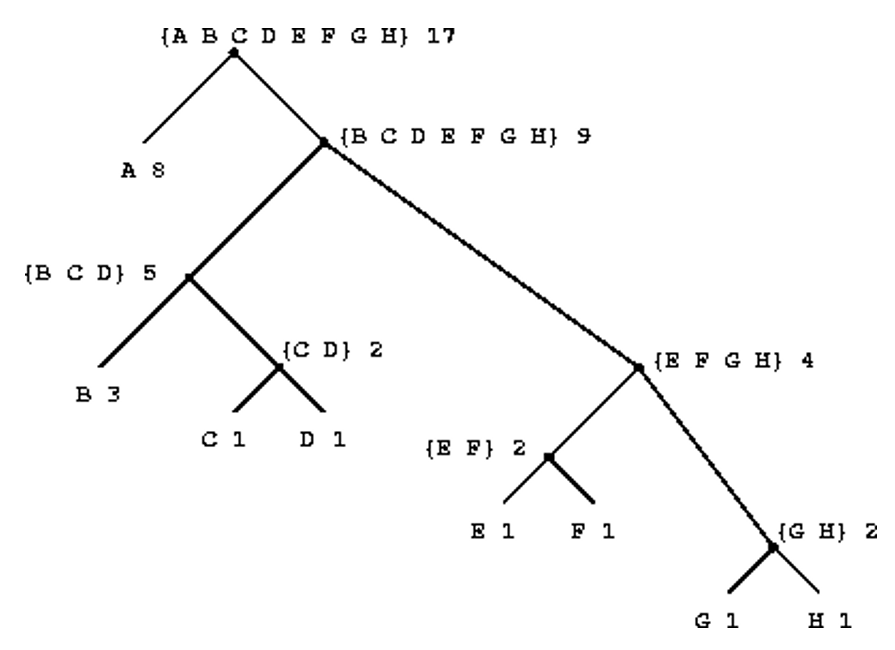
\includegraphics[width=\columnwidth]{images/哈夫曼编码树.png}

\textbf{字符的编码过程:}
从树根开始,每次往包含该字符的子树走。往左子树走,则编码加上比特1,往右子树走,则编码加上比特0

\begin{tabular}{ll}
	A & 0\\
	B & 100\\
	C & 1010\\
	G & 1110\\
	H & 1111\\
	
\end{tabular}

\textbf{字符串编码的解码过程:}从树根开始,在字符串编码中碰到一个0,就往左子树走,碰到1,就往右子树走。走到叶子,即解码出一个字符。然后回到树根重复前面的过程。

10001010

BAC

基本思想:使用频率越高的字符,离树根越近。构造过程和最优二叉树一样

过程:

1. 开始时,若有n个字符,则就有n个结点。每个结点的权值就是字符的频率,每个结点的字符集就是一个字符。

2. 取出权值最小的两个结点,合并为一棵子树。子树的树根的权值为两个结点的权值之和,字符集为两个结点字符集之并。在结点集合中删除取出的两个结点,加入新生成的树根。

3. 如果结点集合中只有一个结点,则建树结束。否则,goto 2

\begin{lstlisting}[style=python]
Initial leaves
{(A 8) (B 3) (C 1) (D 1) (E 1) (F 1) (G 1) (H 1)}Merge
{(A 8) (B 3) ({C D} 2) (E 1) (F 1) (G 1) (H 1)}Merge
{(A 8) (B 3) ({C D} 2) ({E F} 2) (G 1) (H 1)}Merge
{(A 8) (B 3) ({C D} 2) ({E F} 2) ({G H} 2)}Merge
{(A 8) (B 3) ({C D} 2) ({E F G H} 4)}Merge
{(A 8) ({B C D} 5) ({E F G H} 4)} Merge
{(A 8) ({B C D E F G H} 9)}Final merge
{({A B C D E F G H} 17)}

\end{lstlisting}

哈夫曼编码树不唯一

如何快速地在结点集合取出权值最小的两个结点?不要$O(n)$的笨办法。
用"堆",可以做到$O(\log(n))$

\subsection{堆}
\subsubsection{堆的定义}
1) 堆(二叉堆)是一个完全二叉树

2) 堆中任何结点优先级都高于或等于其两个子结点(什么叫优先级高可以自己定义)



3) 一般将堆顶元素最大的堆称为大根堆(大顶堆),堆顶元素最小的堆称为小根堆(小顶堆)

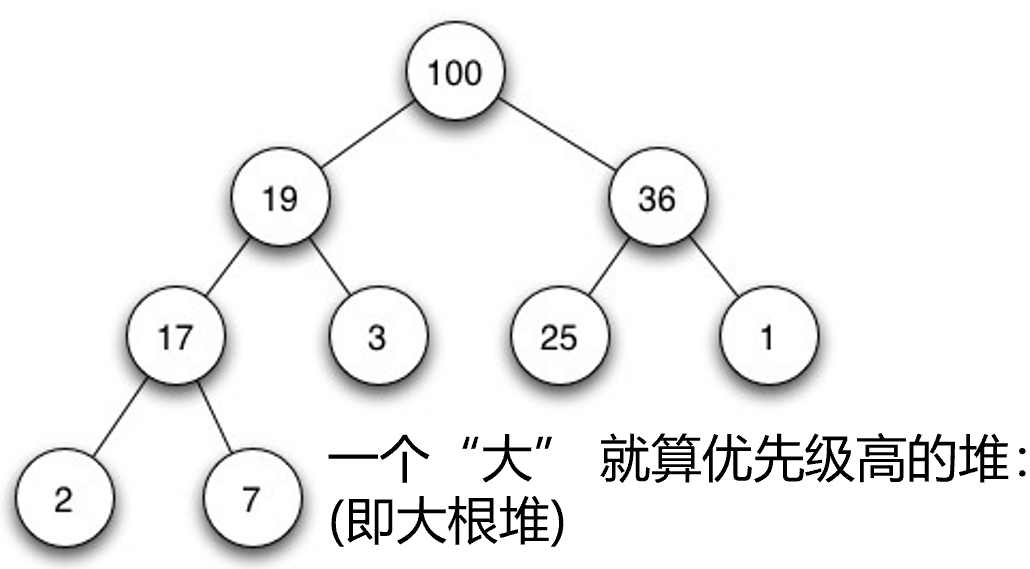
\includegraphics[width=\columnwidth]{images/大根堆.png}

\subsubsection{堆的存储}
用列表存放堆。堆顶元素下标是0。下标为 \verb|i| 的结点,其左右子结点下标分别为 \verb|i*2+1, i*2+2|。

\subsubsection{堆的性质}
1) 堆顶元素是优先级最高的(啥叫优先级高可自定义)

2) 中的任何一棵子树都是堆

3) 往堆中添加一个元素,并维持堆性质,复杂度$O(\log(n))$

4) 删除堆顶元素,剩余元素依然维持堆性质,复杂度$O(\log(n))$

5) 在无序列表中原地建堆,复杂度$O(n)$

\subsubsection{堆的作用}

堆用于需要经常从一个集合中取走(即删除)优先级最高元素,而且还要经常往集合中添加元素的场合(堆可以用来实现优先队列)

可以用堆进行排序,复杂度$O(n\log(n))$,且只需要$O(1)$的额外空间,称为“堆排序”。递归写法需要$O(\log(n))$额外空间,非递归写法需要$O(1)$额外空间。

\subsubsection{堆的操作}
\textbf{添加一个元素}

假设堆存放在列表a中,长度为n

添加元素x到列表a尾部,使其成为a[n]

若x优先级高于其父结点,则令其和父结点交换,直到x优先级不高于其父结点,或x被交换到a[0],变成堆顶为止。此过程称为将x"上移"

x停止交换后,新的堆形成,长度为n+1

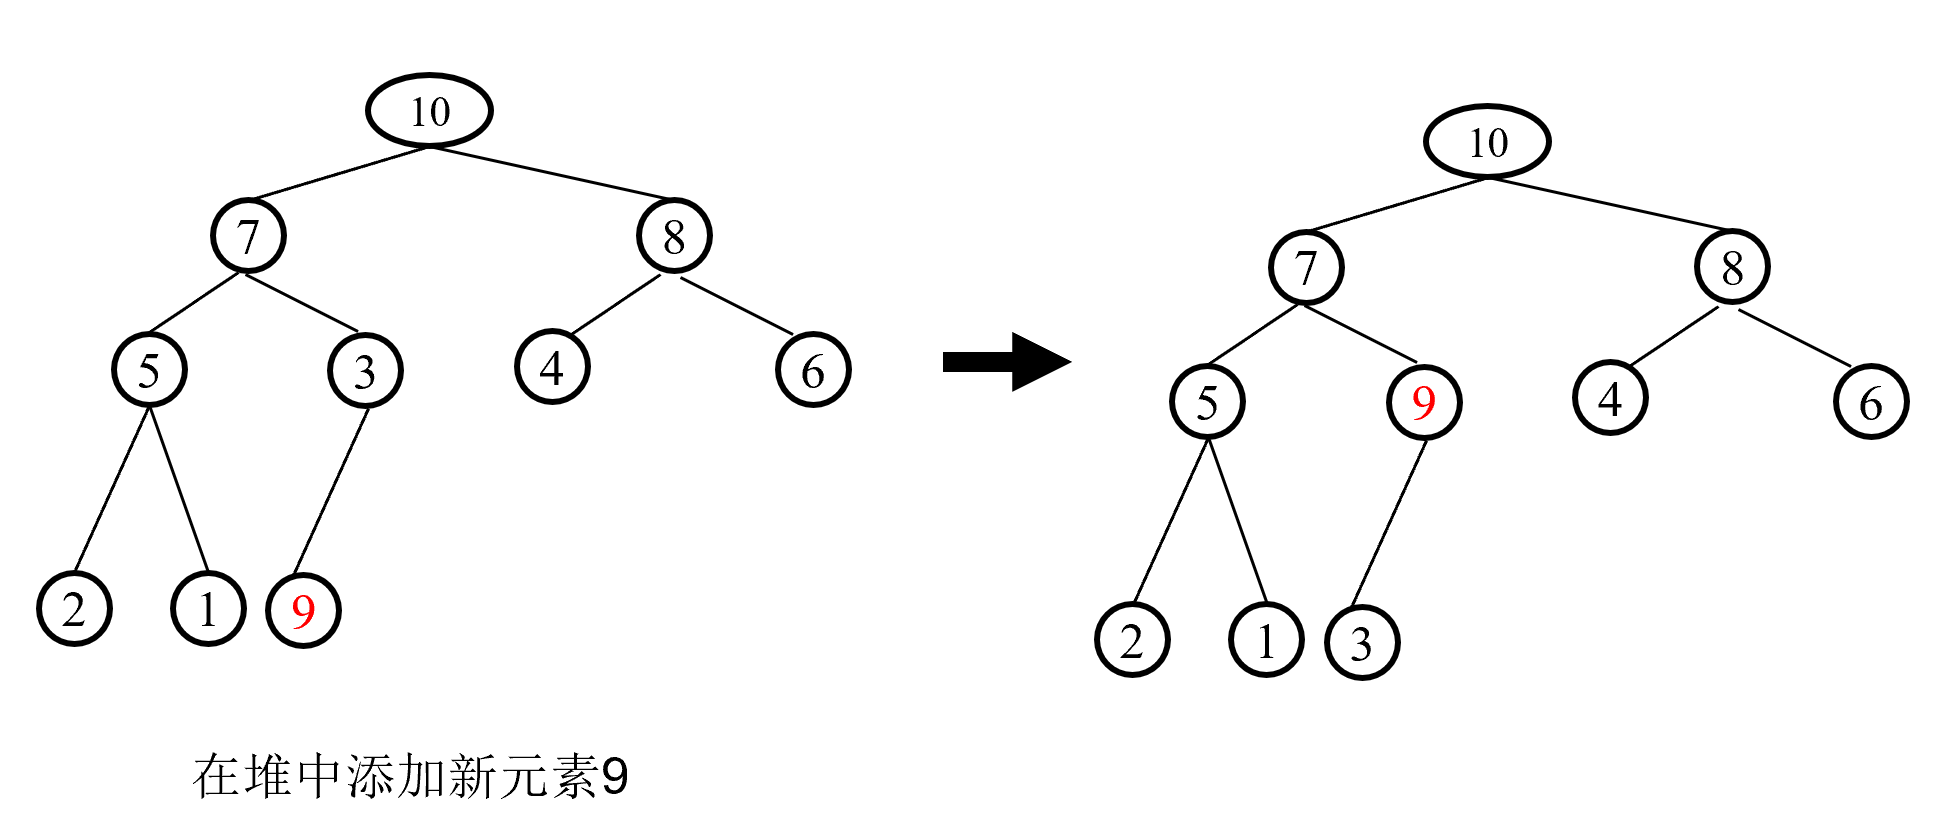
\includegraphics[width=.6\columnwidth]{images/堆中添加元素1.png}
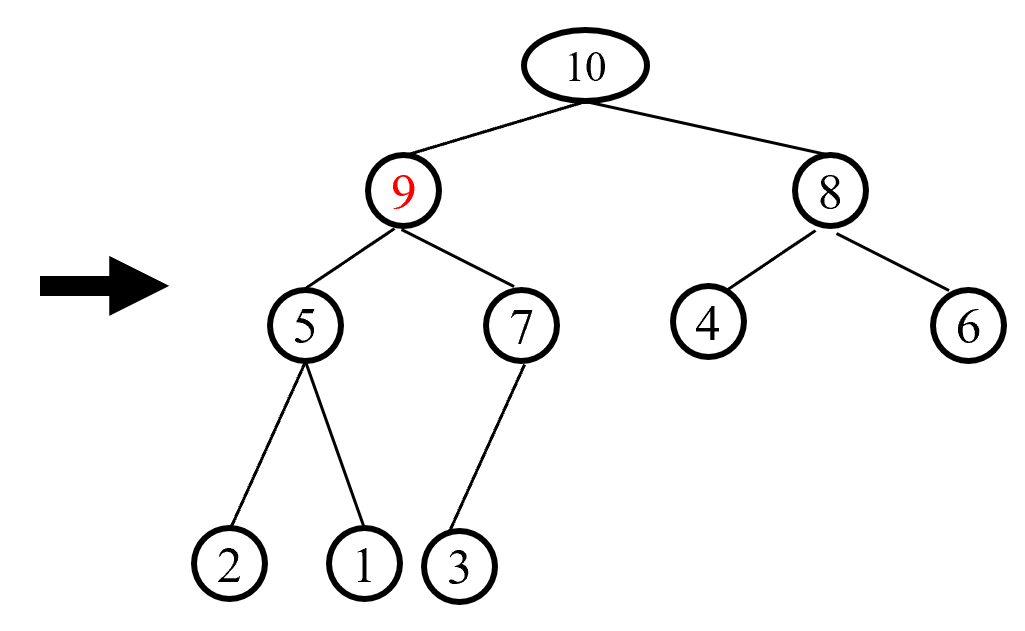
\includegraphics[width=.3\columnwidth]{images/堆中添加元素2.png}


显然,交换过程中,以x为根的子树,一直都是个堆

由于n个元素的完全二叉树高度为$\log_2(n+1)$向上取整,每交换一次x就上升一层,因此上移操作复杂度$O(\log(n))$,即添加元素复杂度$O(\log(n))$

\textbf{删除堆顶元素}
1) 假设堆存放在列表a中,长度为n

2) 将a[0]和a[n-1]交换

3)将a[n-1]删除(pop)

4)记此时的a[0]为x,则将x和它两个儿子中优先级较高的,且优先级高于x的那个交换,直到x变成叶子结点,或者x的儿子优先级都不高于x为止。将此整个过程称为将x"下移"

5) x停止交换后,新的堆形成,长度为n-1

下移过程复杂度为$O(\log(n))$,因此删除堆顶元素复杂度$O(\log(n))$

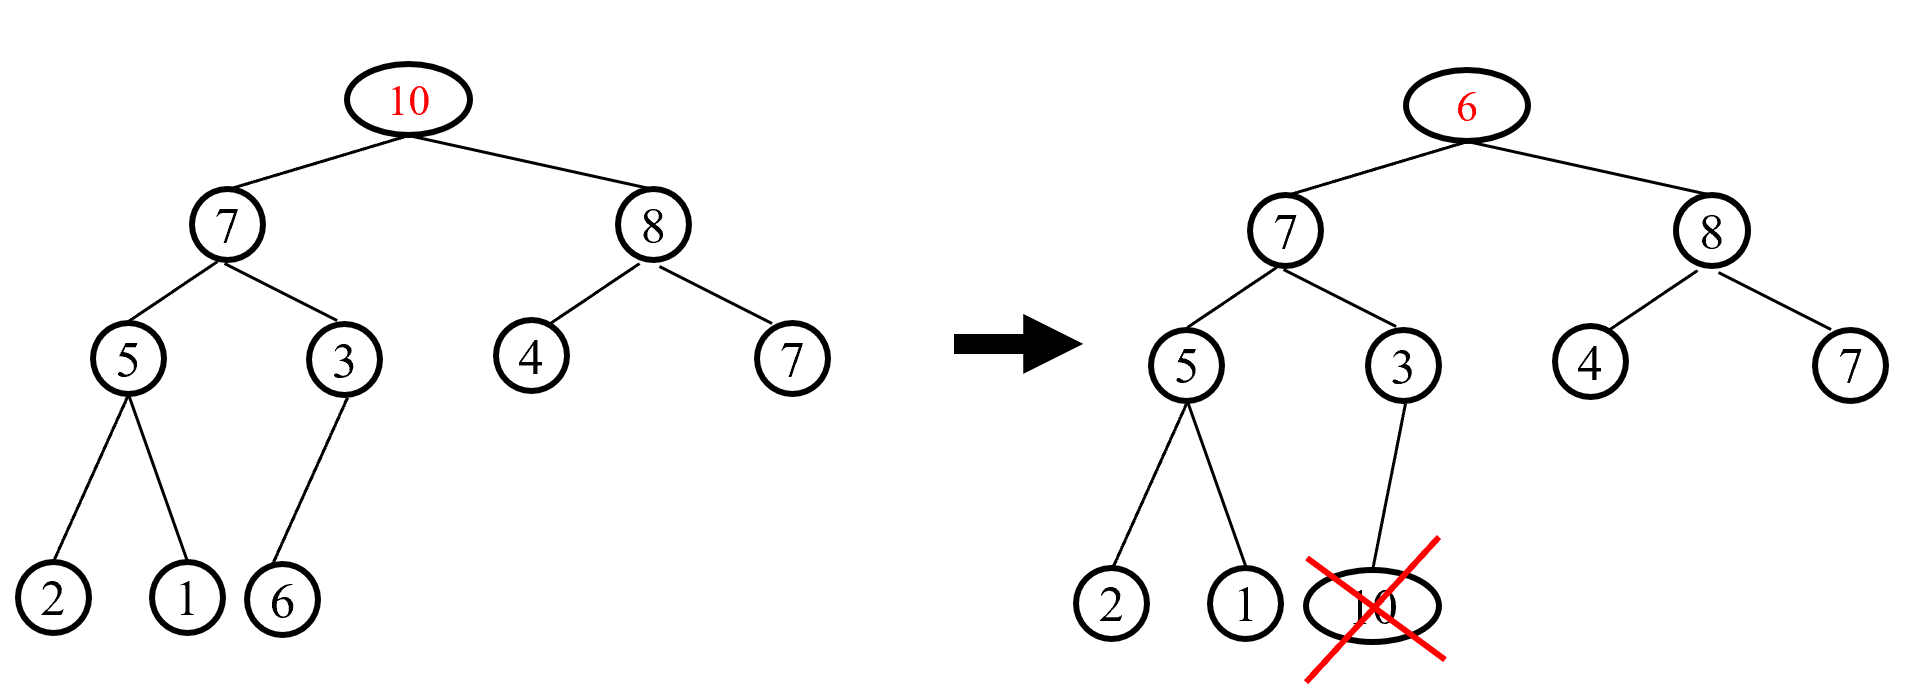
\includegraphics[width=\columnwidth]{images/删除堆顶元素1.png}
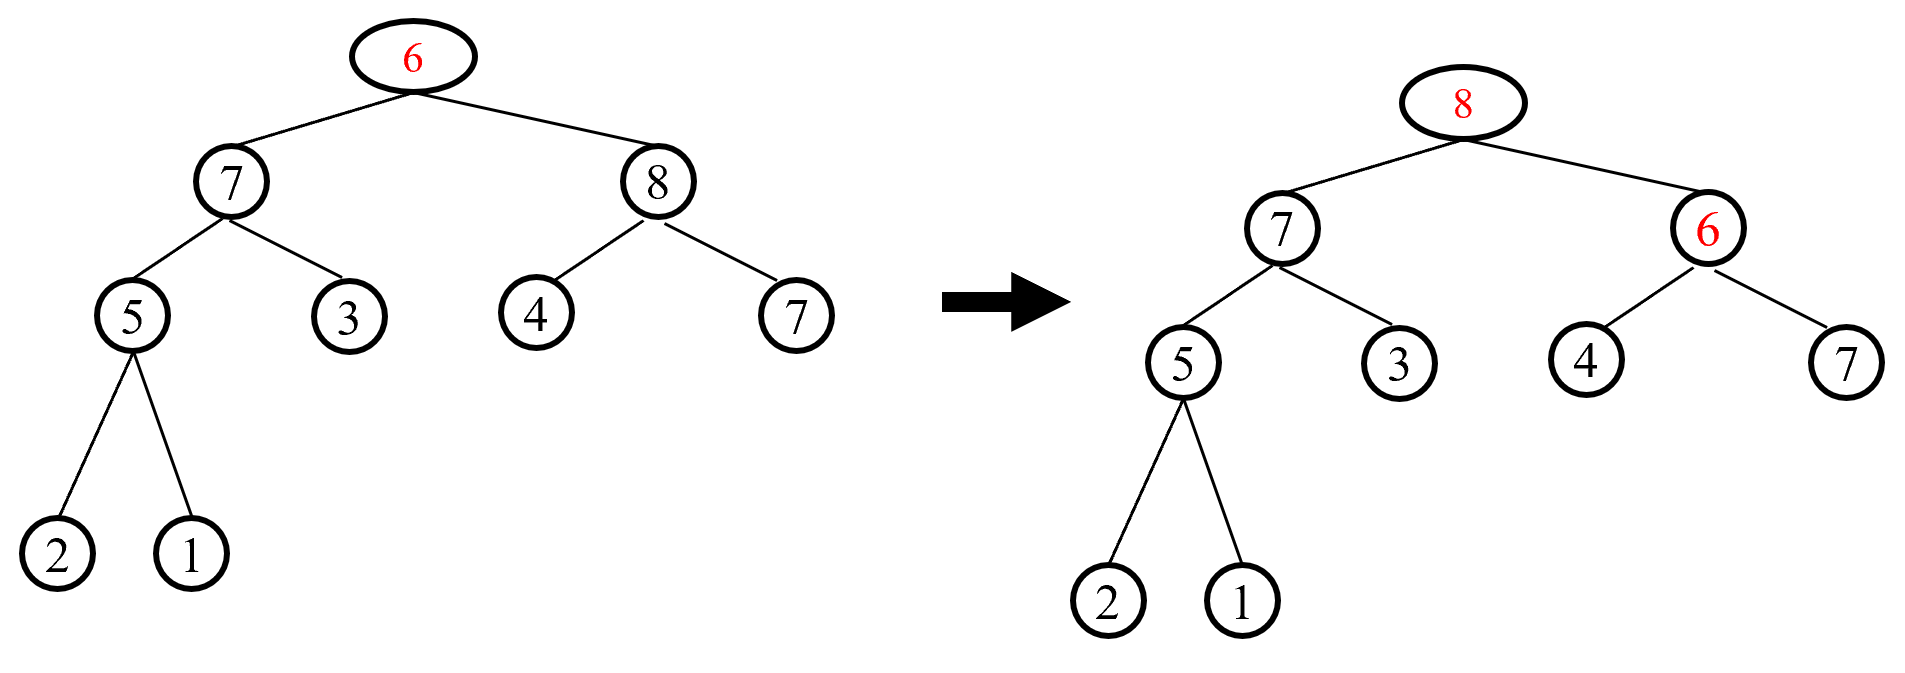
\includegraphics[width=\columnwidth]{images/删除堆顶元素2.png}
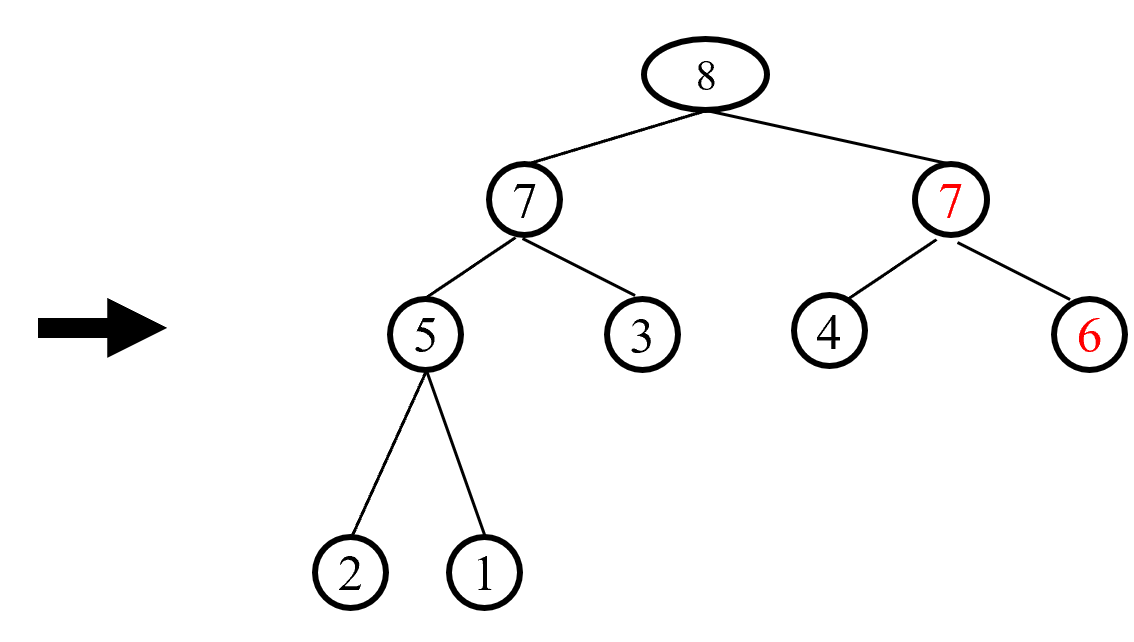
\includegraphics[width=.5\columnwidth]{images/删除堆顶元素3.png}



重要结论:

如果a[i]的两棵子树都是堆,则对a[i]的下移操作完成后,以新a[i]为根的子树会形成堆。

\textbf{建堆}

一个长度为n的列表a,要原地将a变成一个堆

方法:

将a看作一个完全二叉树。假设有H层。根在第0层,第H-1层都是叶子

对第H-2层的每个元素执行下移操作

对第H-3层的每个元素执行下移操作

.....

对第0层的元素执行下移操作

堆即建好。复杂度$O(n)$。

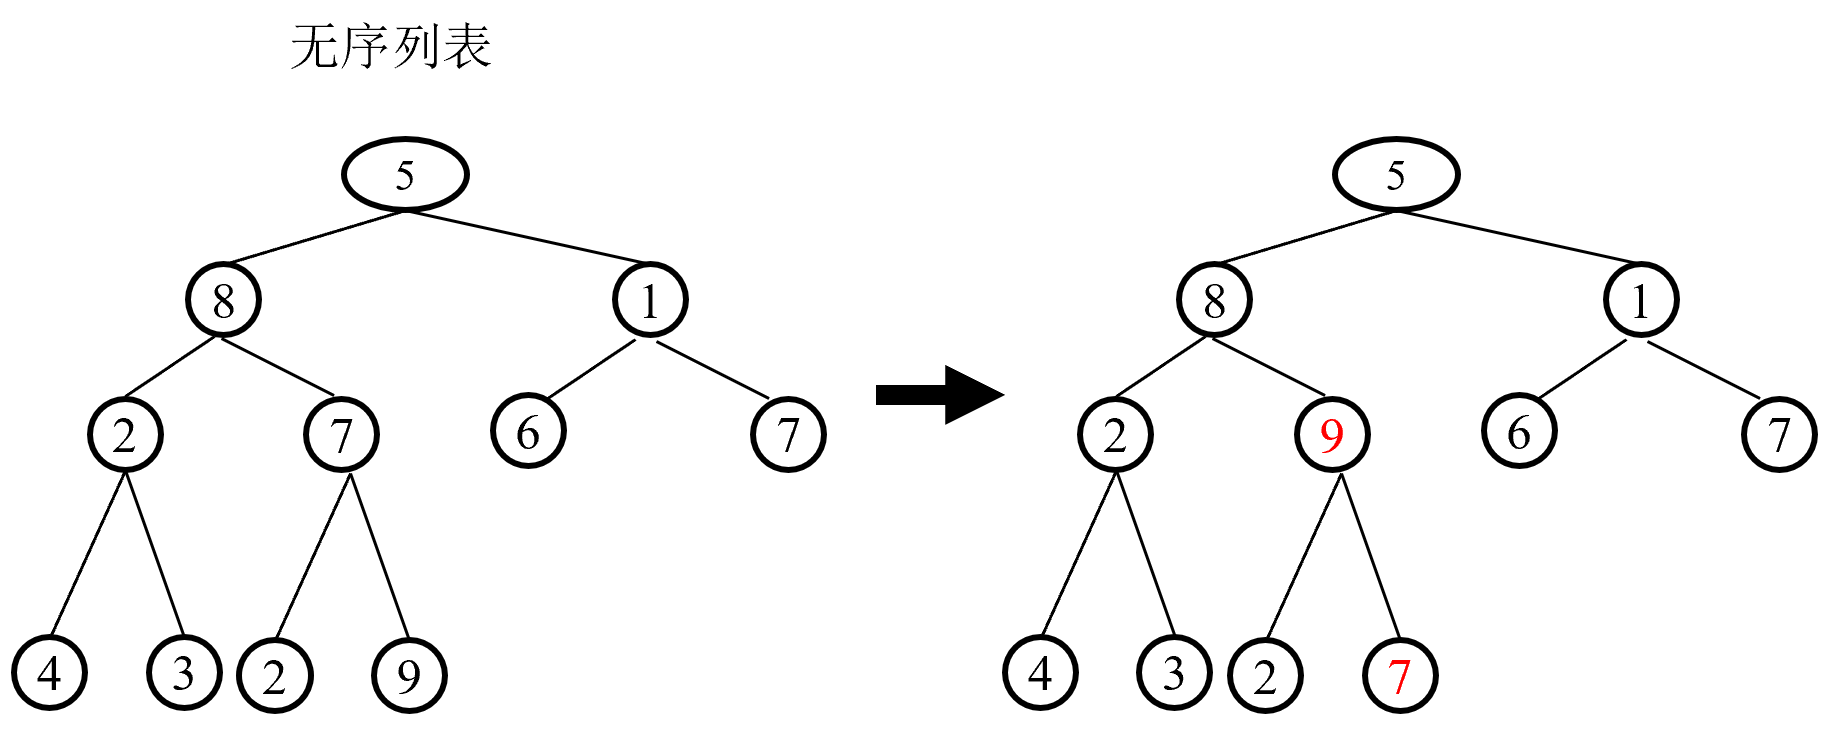
\includegraphics[width=\columnwidth]{images/建堆1.png}
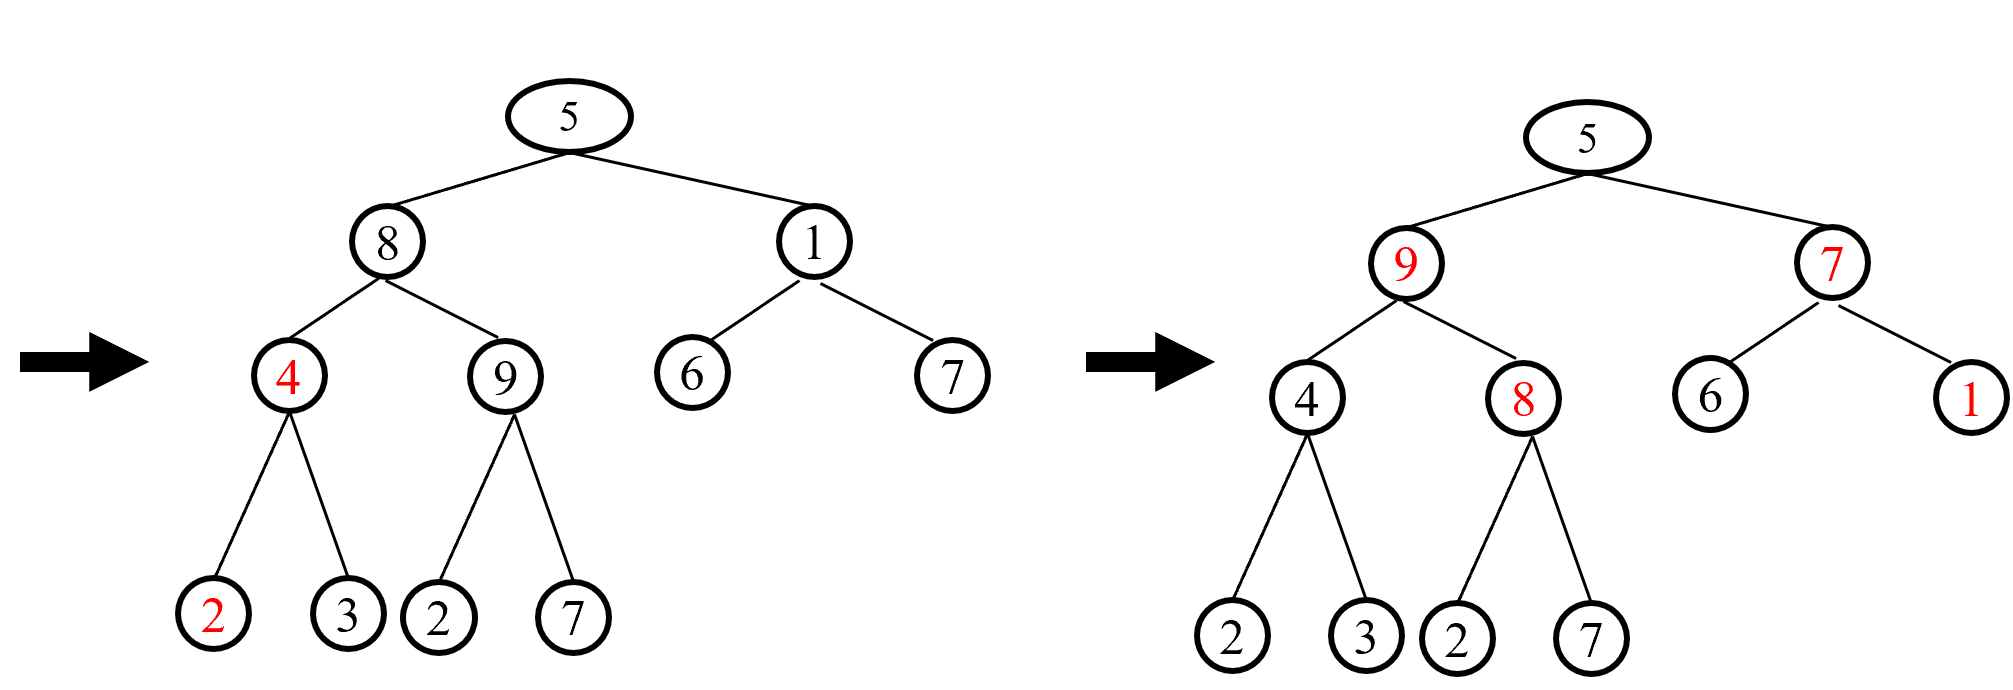
\includegraphics[width=\columnwidth]{images/建堆2.png}
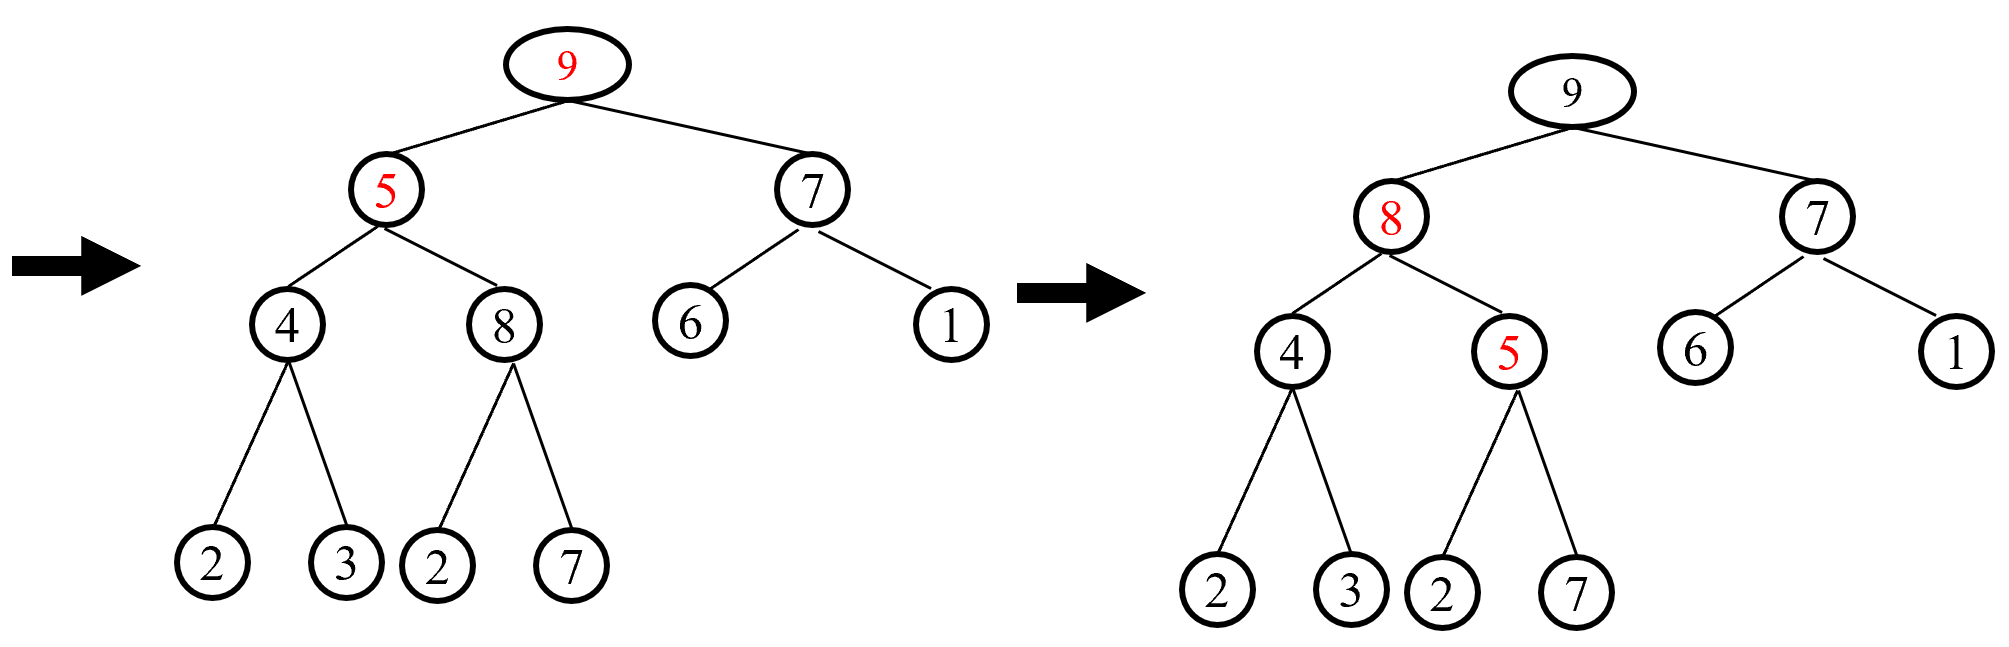
\includegraphics[width=\columnwidth]{images/建堆3.png}
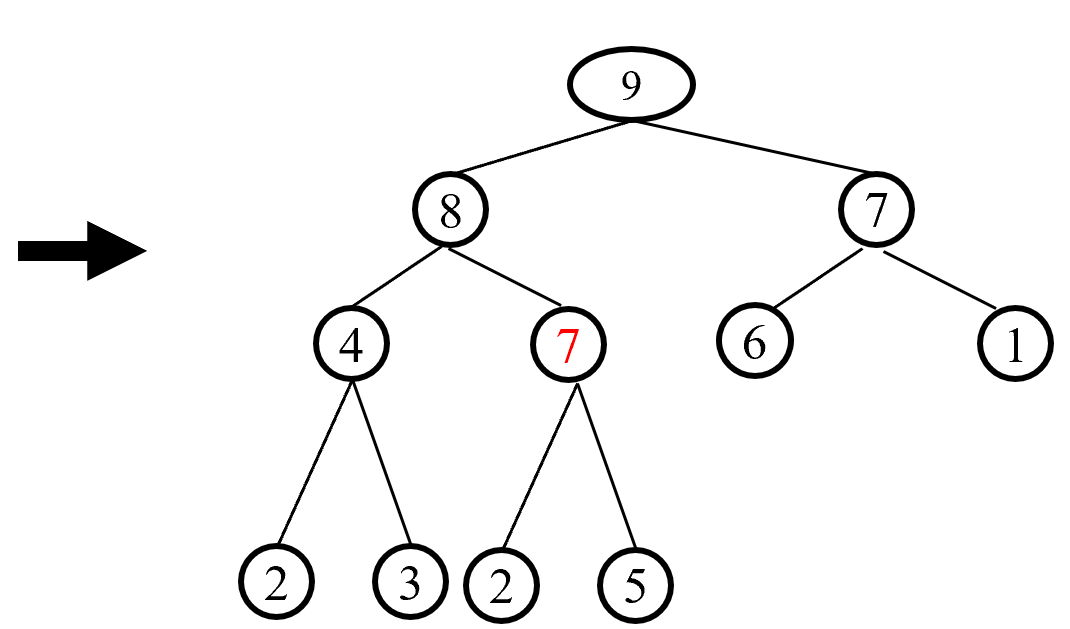
\includegraphics[width=.5\columnwidth]{images/建堆4.png}

\subsubsection{堆的应用}
\textbf{哈夫曼编码树的构造}
\begin{lstlisting}[style=python]
Initial leaves
{(A 8) (B 3) (C 1) (D 1) (E 1) (F 1) (G 1) (H 1)}Merge
{(A 8) (B 3) ({C D} 2) (E 1) (F 1) (G 1) (H 1)}Merge
{(A 8) (B 3) ({C D} 2) ({E F} 2) (G 1) (H 1)}Merge
{(A 8) (B 3) ({C D} 2) ({E F} 2) ({G H} 2)}Merge
{(A 8) (B 3) ({C D} 2) ({E F G H} 4)}Merge
{(A 8) ({B C D} 5) ({E F G H} 4)} Merge
{(A 8) ({B C D E F G H} 9)}Final merge
{({A B C D E F G H} 17)}

\end{lstlisting}
哈夫曼编码树不唯一

用"堆"存放结点集合,便于快速取出最小权值的两个结点,以及加入合并后的新结点。

\textbf{堆排序}

1) 将待排序列表a变成一个堆($O(n)$)

2) 将a[0]和a[n-1]交换,然后对新a[0]做下移,维持前n-1个元素依然是堆。此时优先级最高的元素就是a[n-1]

3) 将a[0]和a[n-2]交换,然后对新a[0]做下移,   维持前n-2个元素依然是堆。此时优先级次高的元素就是a[n-2]

......

直到堆的长度变为1,列表a就按照优先级从低到高排好序了。

整个过程相当不断删除堆顶元素放到a的后部。堆顶元素依次是优先级最高的、次高的....

一共要做$n$次下移,每次下移$O(\log(n))$,因此总复杂度$O(n\log(n))$

如果用递归实现,需要$O(\log(n))$额外栈空间(递归要进行$\log(n)$层)。

如果不用递归实现,需要$O(1)$额外空间。

\subsubsection{堆的实现}

\begin{lstlisting}[style=python]
class Heap:
	def __init__(self,array = [],less = lambda x,y : x < y): 
		#若x为堆顶元素,y为堆中元素,则 less(x,y)为True
		#默认情况下,小的算优先级高 #i的儿子是2*i+1和2*i+2
		self._a = array[:] #array是列表
		self._size = len(array)
		self._less = less 	#less是比较函数
		self.makeHeap()
	def top(self): 
		return self._a[0]
	def pop(self):	#删除堆顶元素
		tmp = self._a[0]
		self._a[0] = self._a[-1]
		self._a.pop()
		self._size -= 1
		self._goDown(0)  #_goDown是下移操作,将a[0]下移
		return tmp
	def append(self,x):	 #往堆中添加x
		self._size += 1
		self._a.append(x)
		self._goUp(self._size-1) #_goUp是上移
	def _goUp(self,i): #将a[i]上移
		#只在append的时候调用,不能直接调用或在别处调用
		#被调用时,以a[i]为根的子树,已经是个堆
		if i == 0:
			return
		f = ( i -1 )// 2  #父结点下标
		if self._less(self._a[i],self._a[f]):
			self._a[i],self._a[f]  = self._a[f],self._a[i]
			self._goUp(f) #a[f]上移
	def _goDown(self,i): #a[i]下移
		#前提:在a[i]的两个子树都是堆的情况下,下移
		if i * 2 + 1 >= self._size: #a[i]没有儿子
			return
		L,R = i * 2 + 1, i * 2 + 2
		if R >= self._size or self._less(self._a[L],self._a[R]):
			s = L
		else:
			s = R
		#上面选择小的儿子
		if self._less(self._a[s],self._a[i]):
			self._a[i],self._a[s] = self._a[s],self._a[i]
			self._goDown(s)
	def makeHeap(self): #建堆
		i = (self._size - 1 - 1) // 2 #i是最后一个叶子的父亲
		for k in range(i,-1,-1):
			self._goDown(k)

	def heapSort(self): #建好堆之后调用,进行堆排序
		for i in range(self._size-1,-1,-1):
			self._a[i],self._a[0] = self._a[0],self._a[i]
			self._size -= 1
			self._goDown(0)
		self._a.reverse()
		return self._a

#下面是堆的用法,不是堆内部的代码
import random
def heapSort(a,less): #对列表a进行堆排序,哪个less哪个排在前面
	hp = Heap(a,less)
	return hp.heapSort()

s = [i for i in range(17)]
random.shuffle(s)
print(s)
h = heapSort(s,lambda x,y : x < y)
print(h)


\end{lstlisting}

\textbf{python中的堆:{\ttfamily heapq}}
\begin{lstlisting}[style=python]
import heapq

heapq.heapify(s)			将列表s变成一个堆
heapq.heappush(s,item)	往已经是堆的s里面添加元素item
heapq.heappop(s)			弹出堆顶元素(会减少s长度)
......

def heapsort(iterable): #iterable是个序列
#函数返回一个列表,内容是iterable中元素排序的结果
	h = []
	for value in iterable:
		h.append(value)
	heapq.heapify(h)
	return [heapq.heappop(h) for i in range(len(h))]
#不便之处:没有设定排序规则的机会。如果要形成大元素在顶的整数堆,只能取-2相反数进堆。出来的时候再取相反数(默认最优是小的)
import heapq
def heapSorted(iterable): #iterable是个序列
#函数返回一个列表,内容是iterable中元素排序的结果,不会改变iterable
	h = []
	for value in iterable:
		h.append(value)
	heapq.heapify(h)
	return [heapq.heappop(h) for i in range(len(h))]

a = (2,13,56,31,5)
print(heapSorted(a)) #>>[2, 5, 13, 31, 56]
print(heapq.nlargest(3,a)) #>>[56, 31, 13]
print(heapq.nlargest(3,a,lambda x:x%10)) #>>[56, 5, 13] 
#取个位数最大的三个
print(heapq.nsmallest(3,a,lambda x:x%10))#>>[31, 2, 13] 
#取个位数最小的三个

\end{lstlisting}

\section{树、森林和并查集}
\subsection{树}
\subsubsection{树的概念}
每个结点可以有任意多棵不相交的子树

子树有序,从左到右依次是子树1,子树2......

二叉树的结点在只有一棵子树的情况下,要区分是左子树还是右子树。树的结点在只有一棵子树的情况下,都算其是第1棵子树 (所以二叉树不是树)

支持广度优先遍历、前序遍历(先处理根结点,再依次处理各个子树)和后序遍历(先依次处理各个子树,再处理根结点),中序遍历无明确定义

\subsubsection{树的性质}


结点度数最多为K的树,第i层最多$K^i$个结点(i从0开始)。

结点度数最多为K的树,高为h时最多有$(K^{h+1} -1 )/(k-1)$ 个结点。

n个结点的K度完全树,高度h是$\log_k (n)$向下取整

n个结点的树有n-1条边

\subsubsection{树的实现}

直观表示法:每个结点有一个变量存放数据,加上一个可变长列表存放所有子结点指针


在不支持可变长列表的语言中,就要想别的办法,比如用二叉树来表示一棵树的儿子-兄弟表示法


父亲表示法:把所有结点编号,在每个结点内记录其父结点编号(用于并查集)


直观表示法
\begin{lstlisting}[style=python]
class Tree:
	def __init__(self,data, *subtrees): #参数个数可变的函数
		#参数subtrees是个元组,其中每个元素都是一个Tree对象
		self.data = data
		self.subtrees = list(subtrees) #self.subtrees是子树列表
	def addSubTree(self,tree): #tree是一个Tree对象
		self.subtrees.append(tree)
	def preorderTraversal(self,op):
		op(self)
		for t in self.subtrees:
			t.preorderTraversal(op)
	def postorderTraversal(self,op):
		for t in self.subtrees:
			t.postorderTraversal(op)
		op(self)
	def printTree(self,level = 0): #输出树的层次结构
		print("\t" * level + str(self.data))
		for t in self.subtrees:
			t.printTree(level+1)

\end{lstlisting}

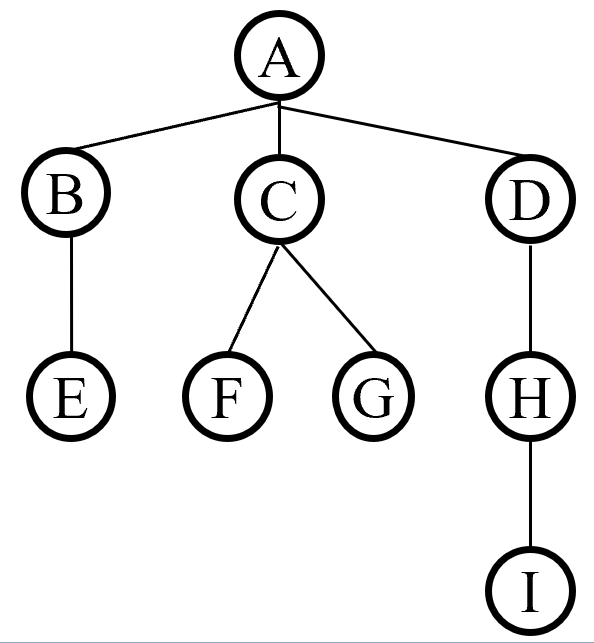
\includegraphics[width=.5\columnwidth]{images/直观表示法.png}
输出形如
\begin{lstlisting}[style=python]
A
	B
		E
	C
		F
		G
	D
		H
			I
\end{lstlisting}

\subsubsection{构建树}
直观表示法
\begin{lstlisting}[style=python]
def buildTree(level): #读取nodesPtr指向的那一行,并建立以其为根的子树
	#该根的层次是level。建好后,令nodesPtr指向该子树的下一行
	global nodesPtr,nodes
	tree = Tree(nodes[nodesPtr][1]) #建根结点
	nodesPtr += 1 #看下一行
	while nodesPtr < len(nodes) and nodes[nodesPtr][0] == level + 1:
		tree.addSubTree(buildTree(level + 1))
	return tree

nodes = []
while True:
	try:
		s = input().rstrip()
		nodes.append((len(s)-1,s.strip()))
	except:
		break
nodesPtr = 0  #表示看到nodes里的第几行
print(nodes)
tree = buildTree(0)
#nodes内容形如:
#[(0, 'A'), (1, 'B'), (2, 'E'), (1, 'C'), (2, 'F'), (2, 'G'), (1, 'D'), (2, 'H'), (3, 'I')]
#元素为(缩进,数据)


\end{lstlisting}

\textbf{儿子-兄弟表示法:}用二叉树B表示一棵树T(二叉树形式表示的树,简称儿子兄弟树)

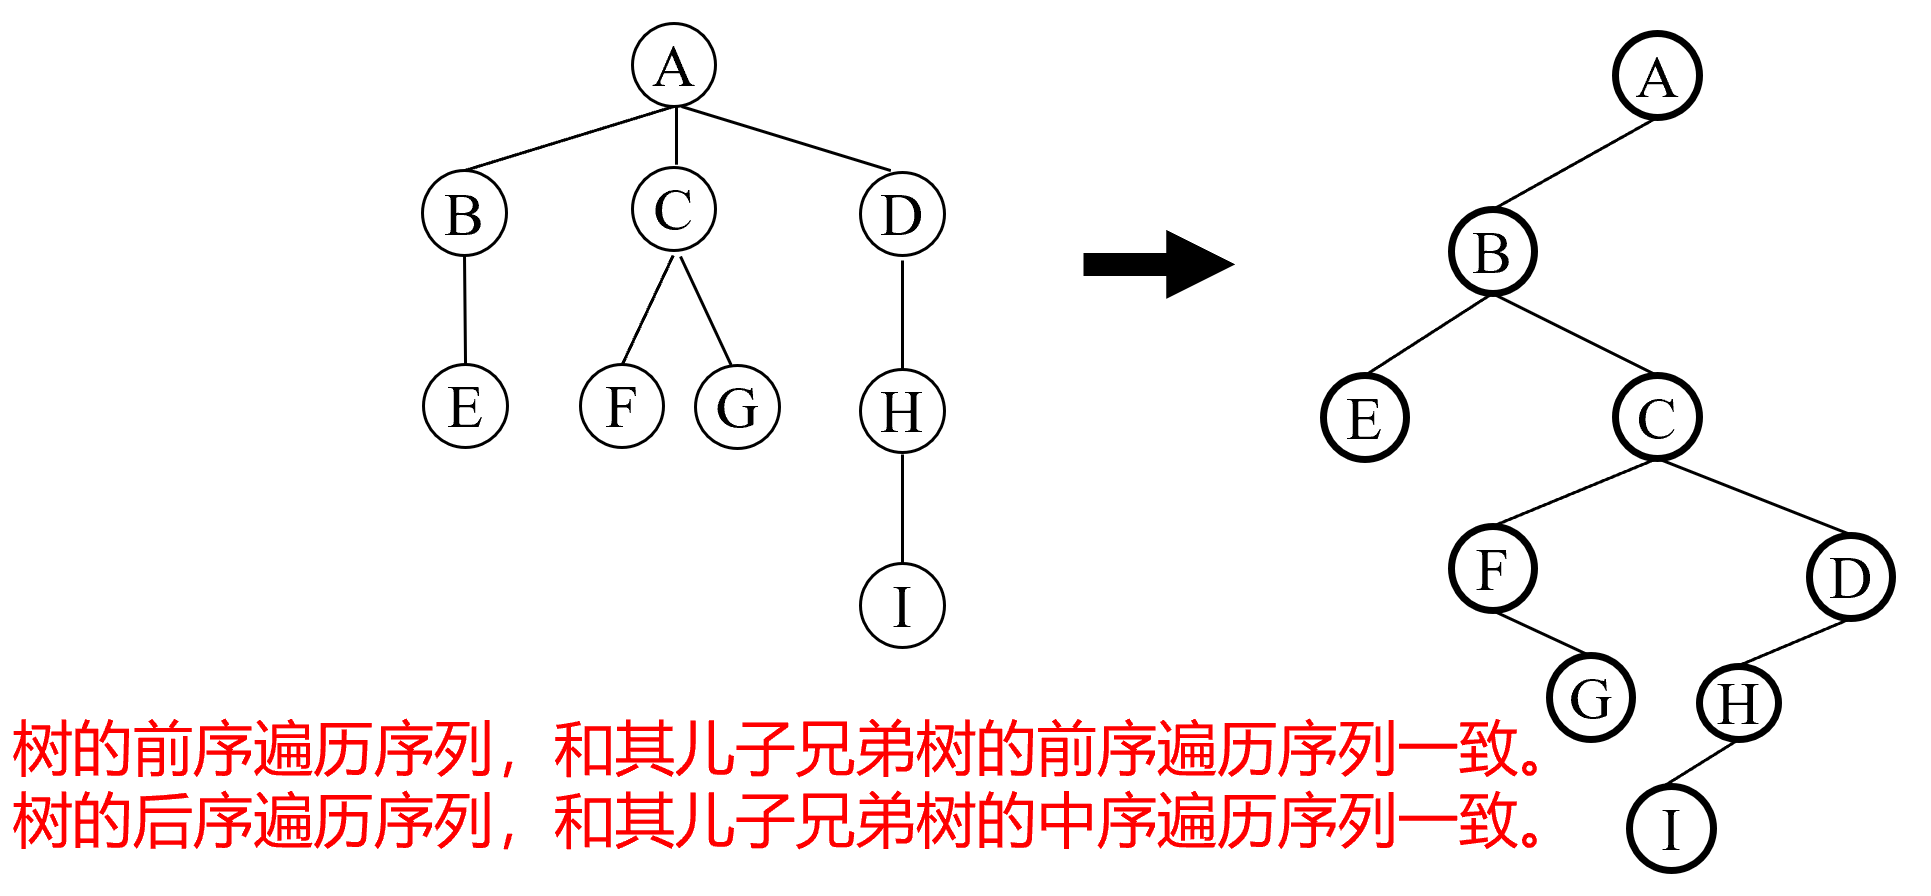
\includegraphics[width=\columnwidth]{images/儿子-兄弟表示法.png}

\textbf{树的直观表示法转儿子兄弟树}
\begin{lstlisting}[style=python]
def treeToBinaryTree(tree):
#直观表示法的树转儿子兄弟树。tree是Tree对象
	bTree = BinaryTree(tree.data) #二叉树讲义中的BinaryTree
	for i in range(len(tree.subtrees)):
		if i == 0:
			tmpTree = treeToBinaryTree(tree.subtrees[i])
			bTree.addLeft(tmpTree)
		else:
			tmpTree.addRight(treeToBinaryTree(tree.subtrees[i]))
			tmpTree = tmpTree.right
	return bTree

#所有结点复制了一份

\end{lstlisting}

\textbf{树的儿子兄弟第表示法转直观表示法}

\begin{lstlisting}[style=python]
def binaryTreeToTree(biTree):
#儿子兄弟树转直观表示法的树转。biTree是BinaryTree对象
	tree = Tree(biTree.data)
	son = biTree.left
	if son:
		tree.addSubTree(binaryTreeToTree(son))
		while son.right:
			tree.addSubTree(binaryTreeToTree(son.right))
			son = son.right
	return tree

#所有结点复制了一份
\end{lstlisting}

\subsection{森林}
\subsubsection{森林的概念}

不相交的树的集合,就是森林

森林有序,有第1棵树、第2棵树、第3棵树之分

森林可以表示为树的列表,也可以表示为一棵二叉树

\subsubsection{森林的二叉树表示法}


1) 森林中第1棵树的根,就是二叉树的根S1,S1及其左子树,是森林的第1棵树的二叉树表示形式

2) S1的右子节S2,以及S2的左子树,是森林的第2棵树的二叉树表示形式

3) S2的右子节S3,以及S3的左子树,是森林的第3棵树的二叉树表示形式

.......

以此类推

\subsubsection{森林的遍历}
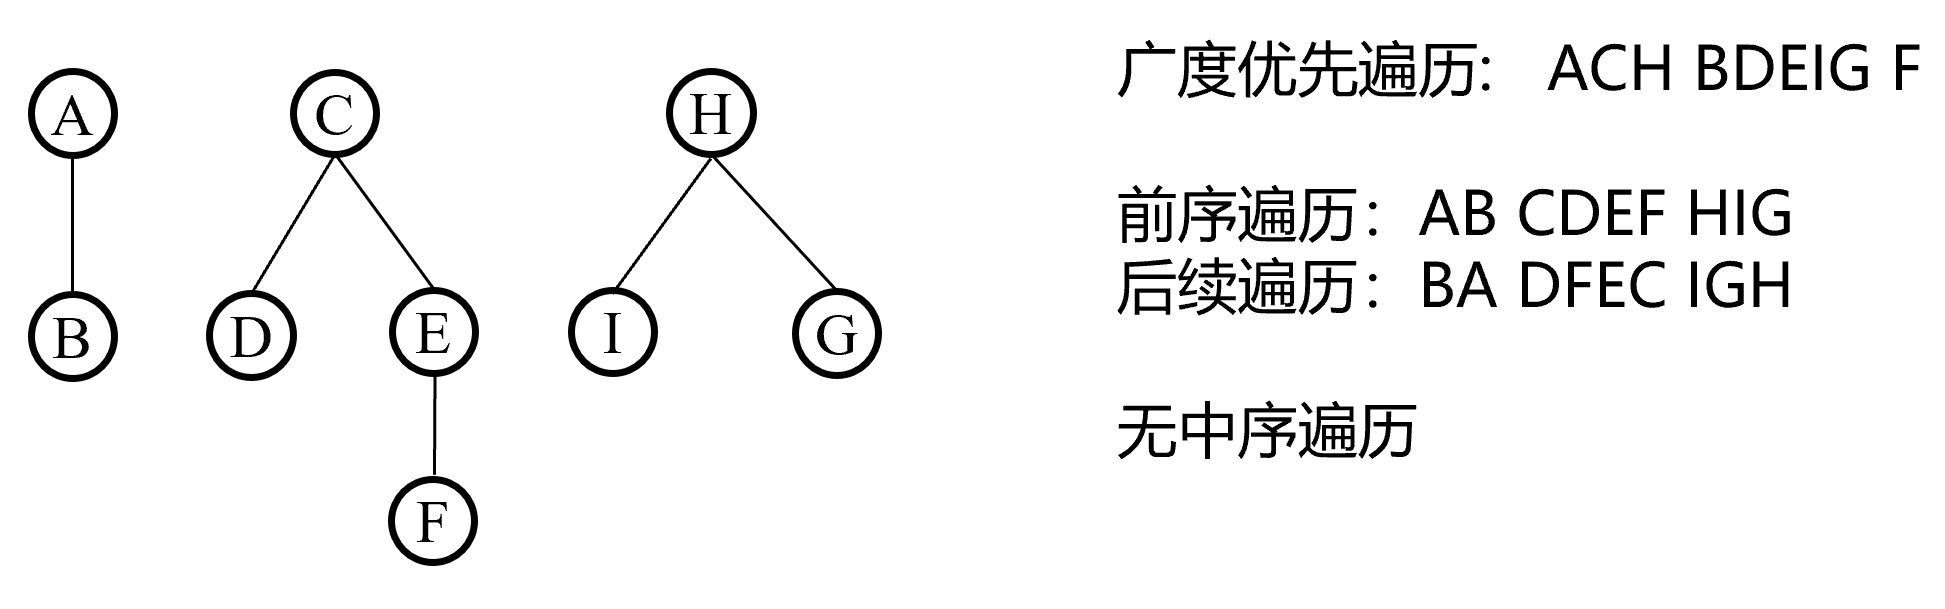
\includegraphics[width=\columnwidth]{images/森林遍历.png}

\subsubsection{森林转二叉树}

\begin{lstlisting}[style=python]
def woodsToBinaryTree(woods):
	#woods是个列表,每个元素都是一棵二叉树形式的树
	
	biTree = woods[0]
	p = biTree
	for i in range(1,len(woods)):
		p.addRight(woods[i])
		p = p.right
	return biTree
#biTree和woods共用结点,执行完后woods的元素不再是原儿子兄弟树

def binaryTreeToWoods(tree):
#tree是以二叉树形式表示的森林
	p = tree
	q = p.right
	p.right = None
	woods = [p]
	if q:
		woods += binaryTreeToWoods(q)
	return woods

#woods是兄弟-儿子树的列表,woods和tree共用结点 
#执行完后tree的元素不再原儿子兄弟树


\end{lstlisting}





\end{multicols}

\end{document}
